\documentclass{mimosis}
\usepackage{vhistory}

\usepackage{metalogo}

\usepackage[final]{pdfpages}

\usepackage{etoolbox}
\usepackage[utf8]{inputenc}

\usepackage{tocloft}
\usepackage[titletoc]{appendix}

\usepackage{graphicx}
\graphicspath{{Pictures_HD/}}

\usepackage[binary-units=true]{siunitx}
\DeclareSIUnit\px{px}

% afkortingen en nomenclatur

\usepackage{acro}
\acsetup{first-style=short}
\DeclareAcronym{ev}{
    short = {EV} ,
    long  = {Electric Vehicle} ,
    foreign  = {Elektrisch Voertuig} ,
    class = {abbrev}
}
\DeclareAcronym{evse}{
    short = {EVSE} ,
    long  = {Electric Cehicle Supply Equipment (EV charger)} ,
    foreign  = {Oplaadpunt} ,
    class = {abbrev}
}
\DeclareAcronym{ccs}{
    short = {CCS} ,
    long  = {Combined Charging System} ,
    foreign  = {Gecombineerd Laadsysteem} ,
    class = {abbrev}
}
\DeclareAcronym{ecu}{
    short = {ECU} ,
    long  = {Electronic Control Unit} ,
    foreign  = {Elektronische Regel Module} ,
    class = {abbrev}
}
\DeclareAcronym{hv}{
    short = {HV} ,
    long  = {High Voltage} ,
    foreign  = {Hoogspanning} ,
    class = {abbrev}
}
\DeclareAcronym{lv}{
    short = {LV} ,
    long  = {Low Voltage} ,
    foreign  = {Laagspanning} ,
    class = {abbrev}
}
\DeclareAcronym{ac}{
    short = {AC} ,
    long  = {Alternating Current} ,
    foreign  = {Wisselstroom} ,
    class = {abbrev}
}
\DeclareAcronym{dc}{
    short = {DC} ,
    long  = {Direct Current} ,
    foreign  = {Gelijkstroom} ,
    class = {abbrev}
}
\DeclareAcronym{can}{
    short = {CAN} ,
    long  = {Controller Area Network} ,
    foreign  = {Controller Gebiedsnetwerk} ,
    class = {abbrev}
}
\DeclareAcronym{bms}{
    short = {BMS} ,
    long  = {Battery Management System} ,
    foreign  = {Batterijbeheer Systeem} ,
    class = {abbrev}
}
\DeclareAcronym{hvil}{
    short = {HVIL} ,
    long  = {High Voltage Interlock Loop} ,
    foreign  = {Hoogspanning Interlock Lus} ,
    class = {abbrev}
}
\DeclareAcronym{hvi}{
    short = {HVIL} ,
    long  = {High Voltage Interlock} ,
    foreign  = {Hoogspanning Interlock} ,
    class = {abbrev}
}
\DeclareAcronym{pwm}{
    short = {PWM} ,
    long  = {Pulse Width Modulation} ,
    foreign  = {Pulsbreedte Modulatie} ,
    class = {abbrev}
}
\DeclareAcronym{soc}{
    short = {SOC} ,
    long  = {State of charge} ,
    foreign  = {Oplaad Niveau} ,
    class = {abbrev}
}
\DeclareAcronym{soh}{
    short = {SOH} ,
    long  = {Conditie} ,
    foreign  = {Oplaadstaat} ,
    class = {abbrev}
}
\DeclareAcronym{rdw}{
    short = {RDW} ,
    long  = {Rijksdienst voor het Wegverkeer} ,
    class = {abbrev}
}
\DeclareAcronym{dbc}{
    short = {DBC} ,
    long  = {CAN bus databases} ,
    foreign  = {CAN-Bus-Databases} ,
    class = {abbrev}
}
\DeclareAcronym{spi}{
    short = {SPI} ,
    long  = {Serial Peripheral Interface} ,
    foreign  = {Seriële Randapparatuur Interface} ,
    class = {abbrev}
}
\DeclareAcronym{ide}{
    short = {IDE} ,
    long  = {Integrated Development Environment} ,
    foreign  = {Geïntegreerde Ontwikkelomgeving} ,
    class = {abbrev}
}
\DeclareAcronym{psu}{
    short = {PSU} ,
    long  = {Power Supply Unit} ,
    foreign  = {Voeding} ,
    class = {abbrev}
}
\DeclareAcronym{usb}{
    short = {USB} ,
    long  = {Universal Serial Bus} ,
    foreign  = {Universelle Seriele Bus} ,
    class = {abbrev}
}
% class `nomencl': nomenclature
% \DeclareAcronym{cpp}{
%     short = {C++} ,
%     long  = {programmeertaal gebaseerd op C} ,
%     sort  = {cpp} ,
%     class = {nomencl}
% }


\setlength{\cftbeforechapskip}{3pt}

\sisetup{%
  detect-all           = true,
  detect-family        = true,
  detect-mode          = true,
  detect-shape         = true,
  detect-weight        = true,
  detect-inline-weight = math,
}

\providecommand{\tightlist}{%
  \setlength{\itemsep}{0pt}\setlength{\parskip}{0pt}}

%%%%%%%%%%%%%%%%%%%%%%%%%%%%%%%%%%%%%%%%%%%%%%%%%%%%%%%%%%%%%%%%%%%%%%%%
% Hyperlinks & bookmarks
%%%%%%%%%%%%%%%%%%%%%%%%%%%%%%%%%%%%%%%%%%%%%%%%%%%%%%%%%%%%%%%%%%%%%%%%

\usepackage[%
  colorlinks = true,
  citecolor  = RoyalBlue,
  linkcolor  = RoyalBlue,
  urlcolor   = RoyalBlue,
  ]{hyperref}

\usepackage{bookmark}


%%%%%%%%%%%%%%%%%%%%%%%%%%%%%%%%%%%%%%%%%%%%%%%%%%%%%%%%%%%%%%%%%%%%%%%%
% Fonts
%%%%%%%%%%%%%%%%%%%%%%%%%%%%%%%%%%%%%%%%%%%%%%%%%%%%%%%%%%%%%%%%%%%%%%%%

\ifxetexorluatex
  \setmainfont{Minion Pro}
\else
  \usepackage[lf]{ebgaramond}
  \usepackage[oldstyle,scale=0.7]{sourcecodepro}
  \singlespacing
\fi

\renewcommand{\th}{\textsuperscript{\textup{th}}\xspace}

%pcb Printed circuit board
%mppt Maximum power point tracking
%spo2 Peripheral oxygen saturation

\newacronym{PCB}{PCB}{Printed circuit board}
\newacronym{MPPT}{MPPT}{Maximum power point tracking}
\newacronym{SPO2}{SPO2}{Peripheral oxygen saturation}
\newacronym{SMD}{SMD}{Surface-mounted Device}
\newacronym{USB}{USB}{Universal Serial Bus}

\makeindex
\makeglossaries

%%%%%%%%%%%%%%%%%%%%%%%%%%%%%%%%%%%%%%%%%%%%%%%%%%%%%%%%%%%%%%%%%%%%%%%%
% Incipit
%%%%%%%%%%%%%%%%%%%%%%%%%%%%%%%%%%%%%%%%%%%%%%%%%%%%%%%%%%%%%%%%%%%%%%%%

\title{Eindverslag \textbf{Stage 3devo}}
\subtitle{Verwarmde behuizing voor het 3D-printen van \ac{hdpe} en \ac{pp}}
\author{Luca van Straaten (18073611)}

\begin{document}

\frontmatter
\begin{titlepage}
    \vspace*{5cm}
    \makeatletter
    \begin{center}
        \begin{Huge}
            \@title
        \end{Huge}\\[0.1cm]
        %
        \begin{Large}
            \@subtitle
        \end{Large}\\
        %
        \emph{door}\\
        \@author
        %
        \vfill
        Dit document is opgesteld voor de stage bij EV Europe. Luca van
        Straaten is een student Elektrotechniek aan de Haagse Hogeschool te
        Delft.\\
        \vspace{.5cm}
        Datum: \today\\
        Versie: 1.0
    \end{center}
    \makeatother
\end{titlepage}

\newpage


\begin{versionhistory}
    \vhEntry{V0.1}{08.09.2021}{Luca}{Document aangemaakt}
    \vhEntry{V0.2}{29.10.2021}{Luca}{Eerste opzet}
    \vhEntry{V1}{17.11.2021}{Luca}{Eerste oplagen}
\end{versionhistory}

\chapter*{Voorwoord}
\addcontentsline{toc}{chapter}{Voorwoord}
%%%%%%%%%%%%%%%%%%%%%%%%%%%%%%%%%%%%%%%%%%%%%%%%%%%%%%%%%%%%%%%%%%%%%%%%

Dit ontwerpdocument is geschreven als documentatie van het tweede stagetraject
van Luca van Straaten.\\\

Dank gaat naar EV Europe voor de mogelijkheid om bij hun mijn tweede stage te
doen, en te leren en groeien als student en als mens.\\\

Dit verslag is bedoeld voor mijn stage beoordeler om te beoordelen of ik
voldoende heb gepresteerd tijdens mijn stage, voor EV Europe en de mensen die
daar werken en verder moeten bouwen op mijn werk en voor Nederlandstalige
geïnteresseerden in het project. Een Engels vertaalde versie van dit verslag is
momenteel niet beschikbaar.\\\

Delft, Januari 2022\\Luca van Straaten

% \chapter{Samenvatting}
\label{Samenvatting}
%%%%%%%%%%%%%%%%%%%%%%%%%%%%%%%%%%%%%%%%%%%%%%%%%%%%%%%%%%%%%%%%%%%%%%%%

\begin{center}
    \begin{minipage}{0.5\textwidth}
        \begin{small}
            Waar in het kort het project van begin tot eind wordt beschreven.
        \end{small}
    \end{minipage}
    \vspace{0.5cm}
\end{center}

Er moest een systeem worden ontworpen om CCS snelladen te implementeren in een
elektrische auto. Er zijn verschillende optie overwogen, zoals zelf alle
elektronica ontwerpen. Maar uiteindelijk is er voor gekozen om een modem van
Zero-EV te gebruiken. Hiervoor moest een communicatie verbinding tussen het BMS
en het modem worden gemaakt. Dit is geïmplementeerd met een CAN bus
controller, maar kan in de toekomst direct vanuit het BMS.

Hoe er tot dit ontwerp, deze optie en het ontwerp van de CAN controller is
gekomen, staat uitgewerkt in dit verslag.

% %%%%%%%%%%%%%%%%%%%%%%%%%%%%%%%%%%%%%%%%%%%%%%%%%%%%%%%%%%%%%%%%%%%%%%%%
% \section{Vooraf}
% %%%%%%%%%%%%%%%%%%%%%%%%%%%%%%%%%%%%%%%%%%%%%%%%%%%%%%%%%%%%%%%%%%%%%%%%

% Bepaalen wat er moet worden gedaan en een plan van aanpak en een plan van eisen opstellen. 

% %%%%%%%%%%%%%%%%%%%%%%%%%%%%%%%%%%%%%%%%%%%%%%%%%%%%%%%%%%%%%%%%%%%%%%%%
% \section{Tijdens het project}
% %%%%%%%%%%%%%%%%%%%%%%%%%%%%%%%%%%%%%%%%%%%%%%%%%%%%%%%%%%%%%%%%%%%%%%%%

% Onderzoek doen naar de mogelike opties en die implementeeren.

% %%%%%%%%%%%%%%%%%%%%%%%%%%%%%%%%%%%%%%%%%%%%%%%%%%%%%%%%%%%%%%%%%%%%%%%%
% \section{Testen van het product}
% %%%%%%%%%%%%%%%%%%%%%%%%%%%%%%%%%%%%%%%%%%%%%%%%%%%%%%%%%%%%%%%%%%%%%%%%

% langs laaders 

%\begingroup
%    \let\clearpage\relax
%    \glsaddall
%    \printglossary[type=\acronymtype]
%    \addcontentsline{toc}{chapter}{Acroniemen}
%\endgroup
\newpage
\tableofcontents
\newpage
\phantomsection
\addcontentsline{toc}{chapter}{\listfigurename}
\listoffigures

\printacronyms[include=abbrev,name=Lijst van afkortingen]
\printacronyms[include=nomencl,name=Lijst van begrippen]

\chapter{Inleiding}
\label{inleiding}
%%%%%%%%%%%%%%%%%%%%%%%%%%%%%%%%%%%%%%%%%%%%%%%%%%%%%%%%%%%%%%%%%%%%%%%%

\begin{center}
    \begin{minipage}{0.5\textwidth}
        \begin{small}
            Waar de reden tot creatie van dit verslag worden blootgelegd, de
            opdracht en het probleem worden beschreven en achtergrondinformatie
            word gegeven.
        \end{small}
    \end{minipage}
    \vspace{0.5cm}
\end{center}

\noindent EV Europe is een bedrijf dat werkt met klanten die gebruik willen
maken van de nieuwste technieken op het gebied van elektrische auto's. Zo word
er vaak door de klanten gevraagd of moderne snufjes kunnen woorden ingebouwd in
hun auto. Recent was dat de vraag om langs de snelweg aan een snel laad paal te
kunnen laadden. Deze palen (of \ac{evse}) maken in europa gebruik van het \ac{ccs}
protocol \cite{Directive_2014/94/EU}. Dus EV Europe is gaan onderzoeken of het
gebruik van deze \ac{ccs} snel laad palen een optie is voor de klanten en wat er
voor nodig is om dit te bereiken.

%%%%%%%%%%%%%%%%%%%%%%%%%%%%%%%%%%%%%%%%%%%%%%%%%%%%%%%%%%%%%%%%%%%%%%%%
\section{Achtergrond electrichen auto's}
%%%%%%%%%%%%%%%%%%%%%%%%%%%%%%%%%%%%%%%%%%%%%%%%%%%%%%%%%%%%%%%%%%%%%%%%

Er zijn grofweg twee soorten electrice autos (\ac{ev}), plug-in elektrische auto's en
hybride auto's. Plug-in elektrische auto's zijn auto's die aleen electrise
rijden, en hybride auto's zijn auto's die zowel electrich en op
verbrandingsmotor rijden (er zijn nog meer onnderschijdingen zoals onderandenen
plug-in hybrid en waterstof autos die niet van toepassing zijn op dit verslag).

EV Europe is vooral geïnterneerd in de eerste soort, de plug-in elektrische
auto's. De plug-in elektrische auto's zijn auto's met een volledig elektrische
aandrijflijn, en die dus ook elektrisch moeten woorden opgeladen. De
aandrijflijn van deze auto's bestaat uit een accupakket, een motorcontroller,
en een elektromotor. De overigen mechanische componenten van de aandrijflijn
zijn vrijwel gelijk aan die van een interne verbrandingsmotor auto.

In de laatset jaaren is de hoeveelhijd electriche autos op de markt hard aan
het groeien. Tevens de infrastruktuur, zoals (snel)laaders. 

%%%%%%%%%%%%%%%%%%%%%%%%%%%%%%%%%%%%%%%%%%%%%%%%%%%%%%%%%%%%%%%%%%%%%%%%
\subsection{Laadden van elektricien auto's}
%%%%%%%%%%%%%%%%%%%%%%%%%%%%%%%%%%%%%%%%%%%%%%%%%%%%%%%%%%%%%%%%%%%%%%%%

Het laaden van EV's gaat wereldwijd door middel van verschillende standaarden,
maar in europa hebben het \ac{ccs} systeem geadopteerd. Ondanks de andere
standaarden die nogsteeds hier en daar ondersteund woorden, focusen we ons in
de verslag volledig op de \ac{ccs} systeem.

%%%%%%%%%%%%%%%%%%%%%%%%%%%%%%%%%%%%%%%%%%%%%%%%%%%%%%%%%%%%%%%%%%%%%%%%
\subsection{\ac{ccs} laadden}
%%%%%%%%%%%%%%%%%%%%%%%%%%%%%%%%%%%%%%%%%%%%%%%%%%%%%%%%%%%%%%%%%%%%%%%%

\ac{ccs} laaden kan met AC en met DC, afhankelijk van de \ac{evse} en de opties
op de auto kan er AC of DC woorden gelaaden. AC laaden staat wel beschreven in
de \ac{ccs} standaard, echter word het ac laaden met de type 2 stekker vaak
niet \ac{ccs} genoemd maar gewoon AC. Er zijn dus twee soorten \ac{ccs}
laadden: AC en DC.

Er zijn ook twee soorten stekkers (de kant van de \ac{evse}) en twee soorten
inlest (de kant van de \ac{ev}). de Combo 2 stekker (zie figuur
\ref{fig:CCS_combo2_outlet}) ondersteund aleen DC laaden, maar de Combo 2 inlet
(zie figuur \ref{fig:CCS_combo2_inlet}) ondersteund over het algemeen zowel AC
als DC laad. verder zijn de type 2 stekker (zie figuur
\ref{fig:AC_type2_inlet_outlet}) en inlet (zie figuur
\ref{fig:AC_type2_inlet_outlet}) alleen voor AC laaden

\begin{figure}[h]
    \centering
    \begin{minipage}{0.45\textwidth}
        \centerline{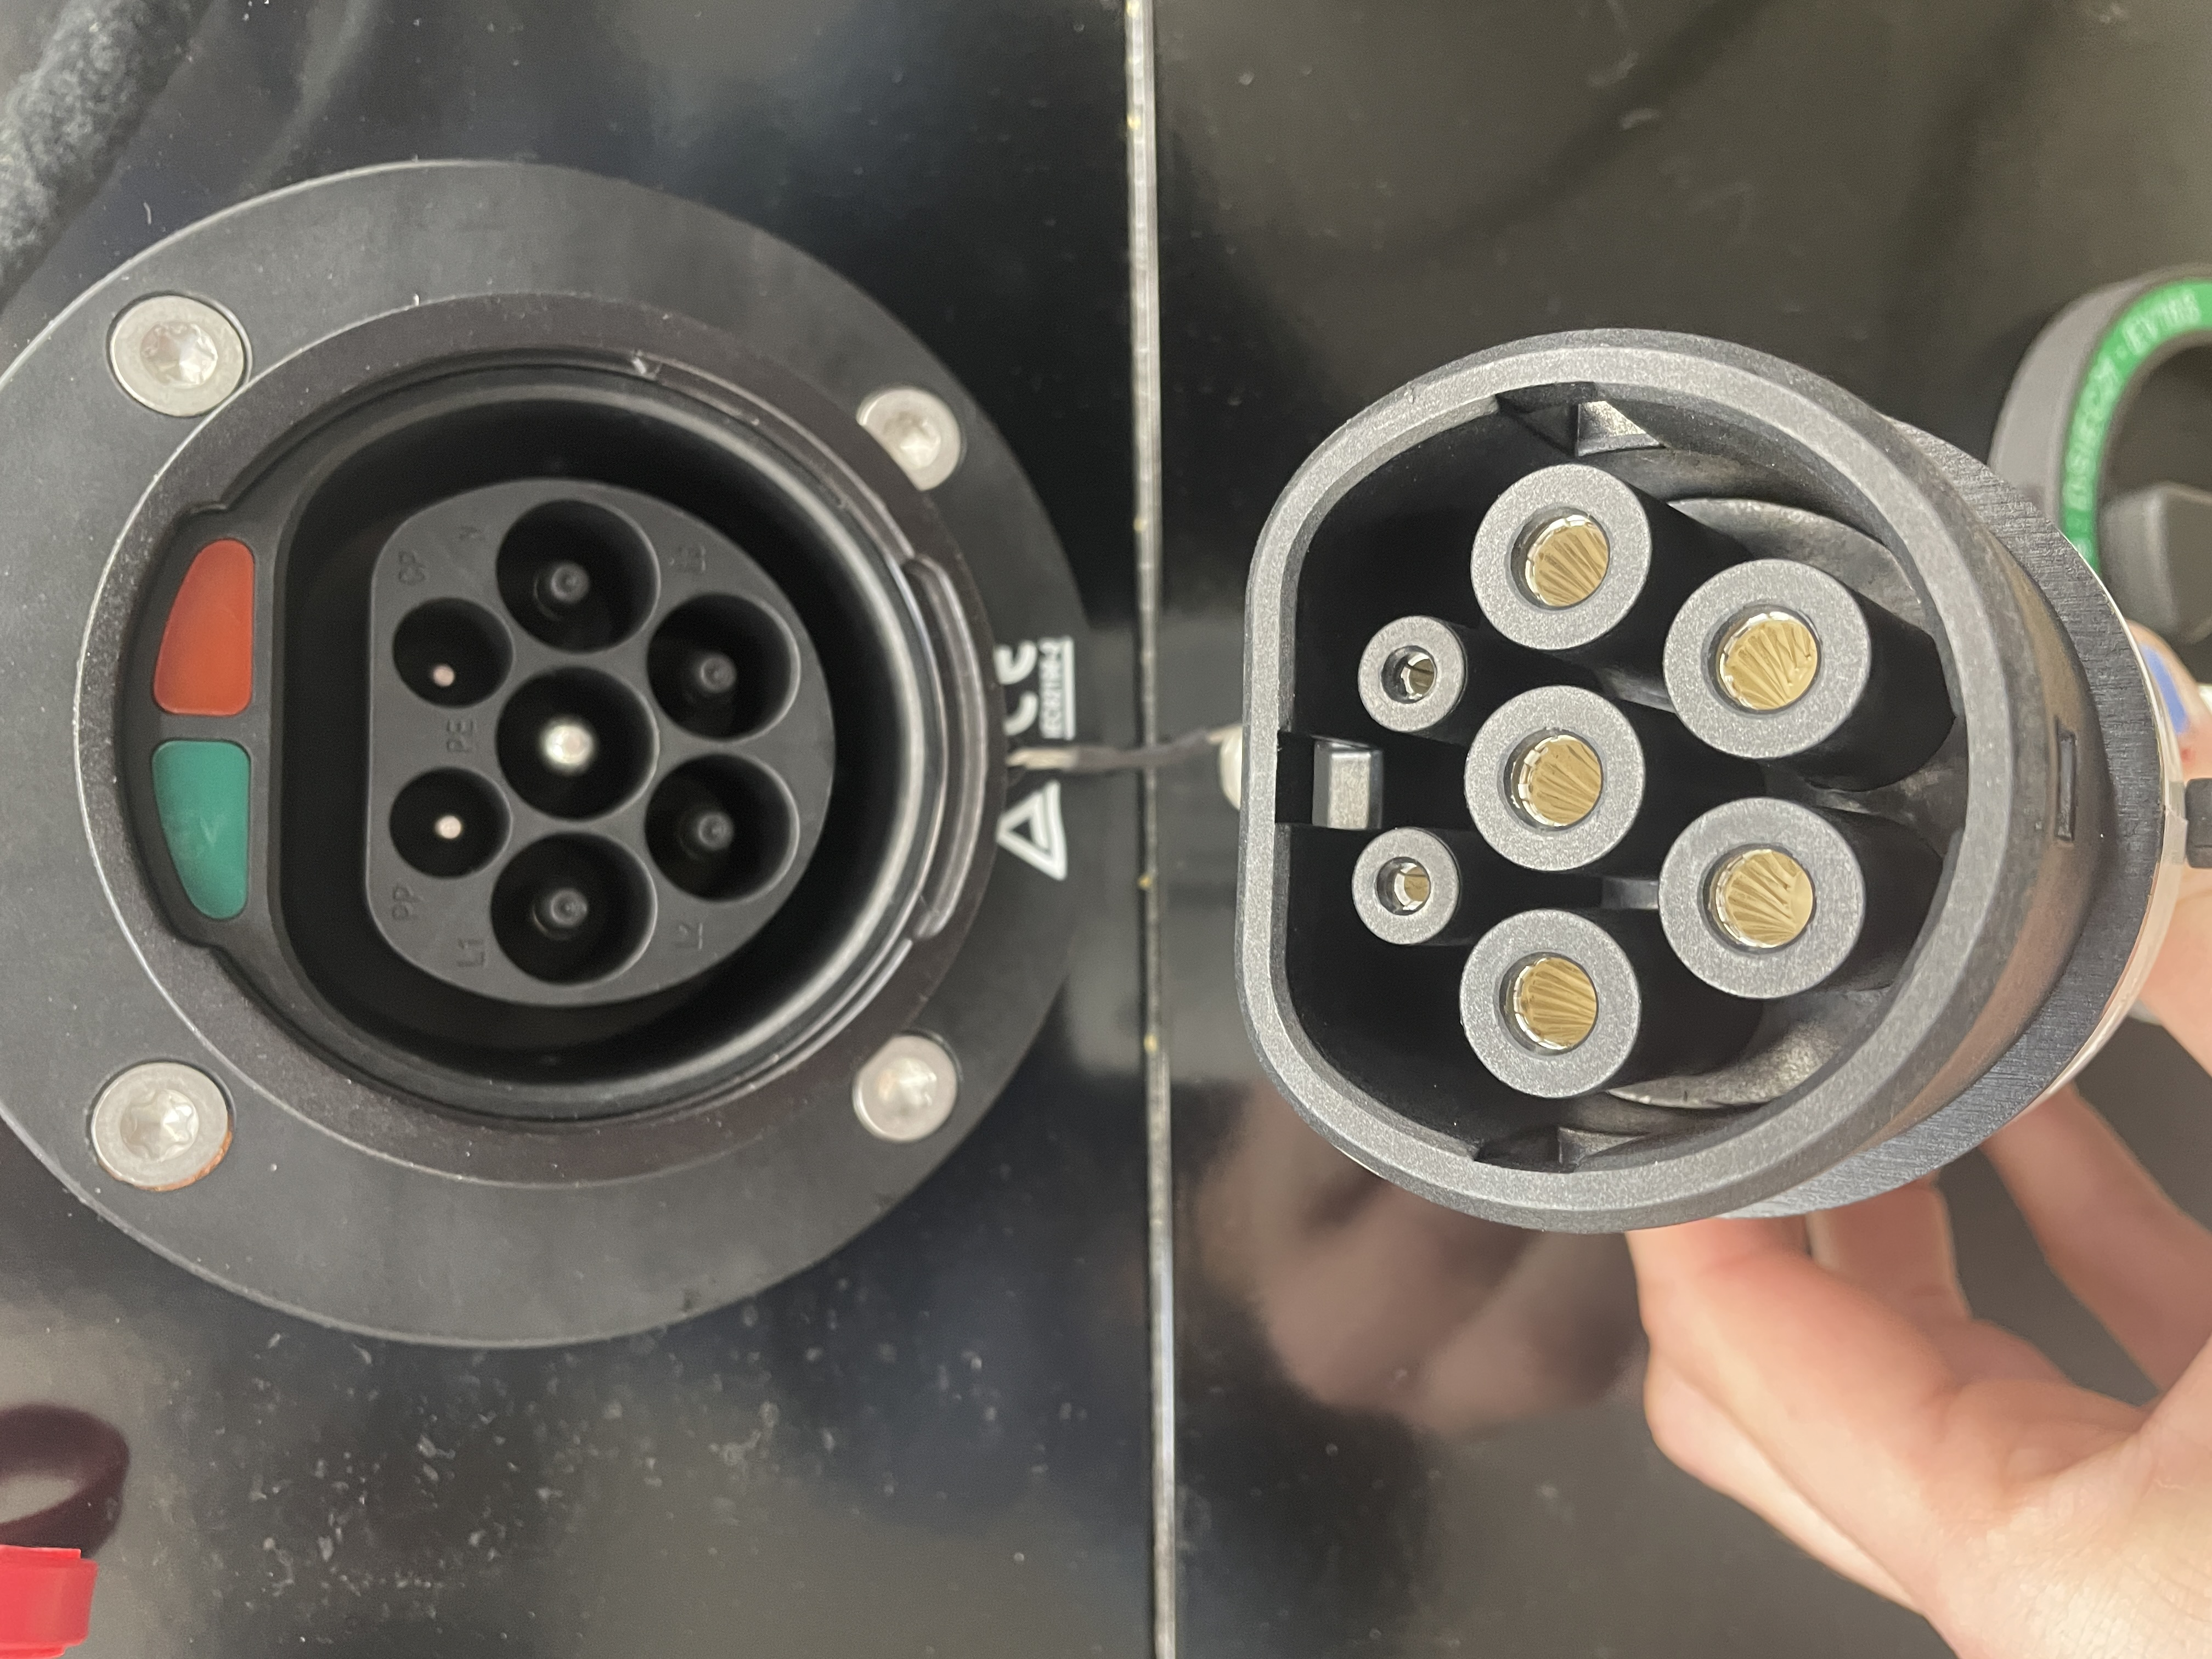
\includegraphics[width=0.9\textwidth,angle=-90]{AC_type2_inlet_outlet}}
        \caption{AC Type 2 inlet (boven) en outlet (onder)}
        \label{fig:AC_type2_inlet_outlet}
    \end{minipage}\hfill
    \begin{minipage}{0.45\textwidth}
        \centerline{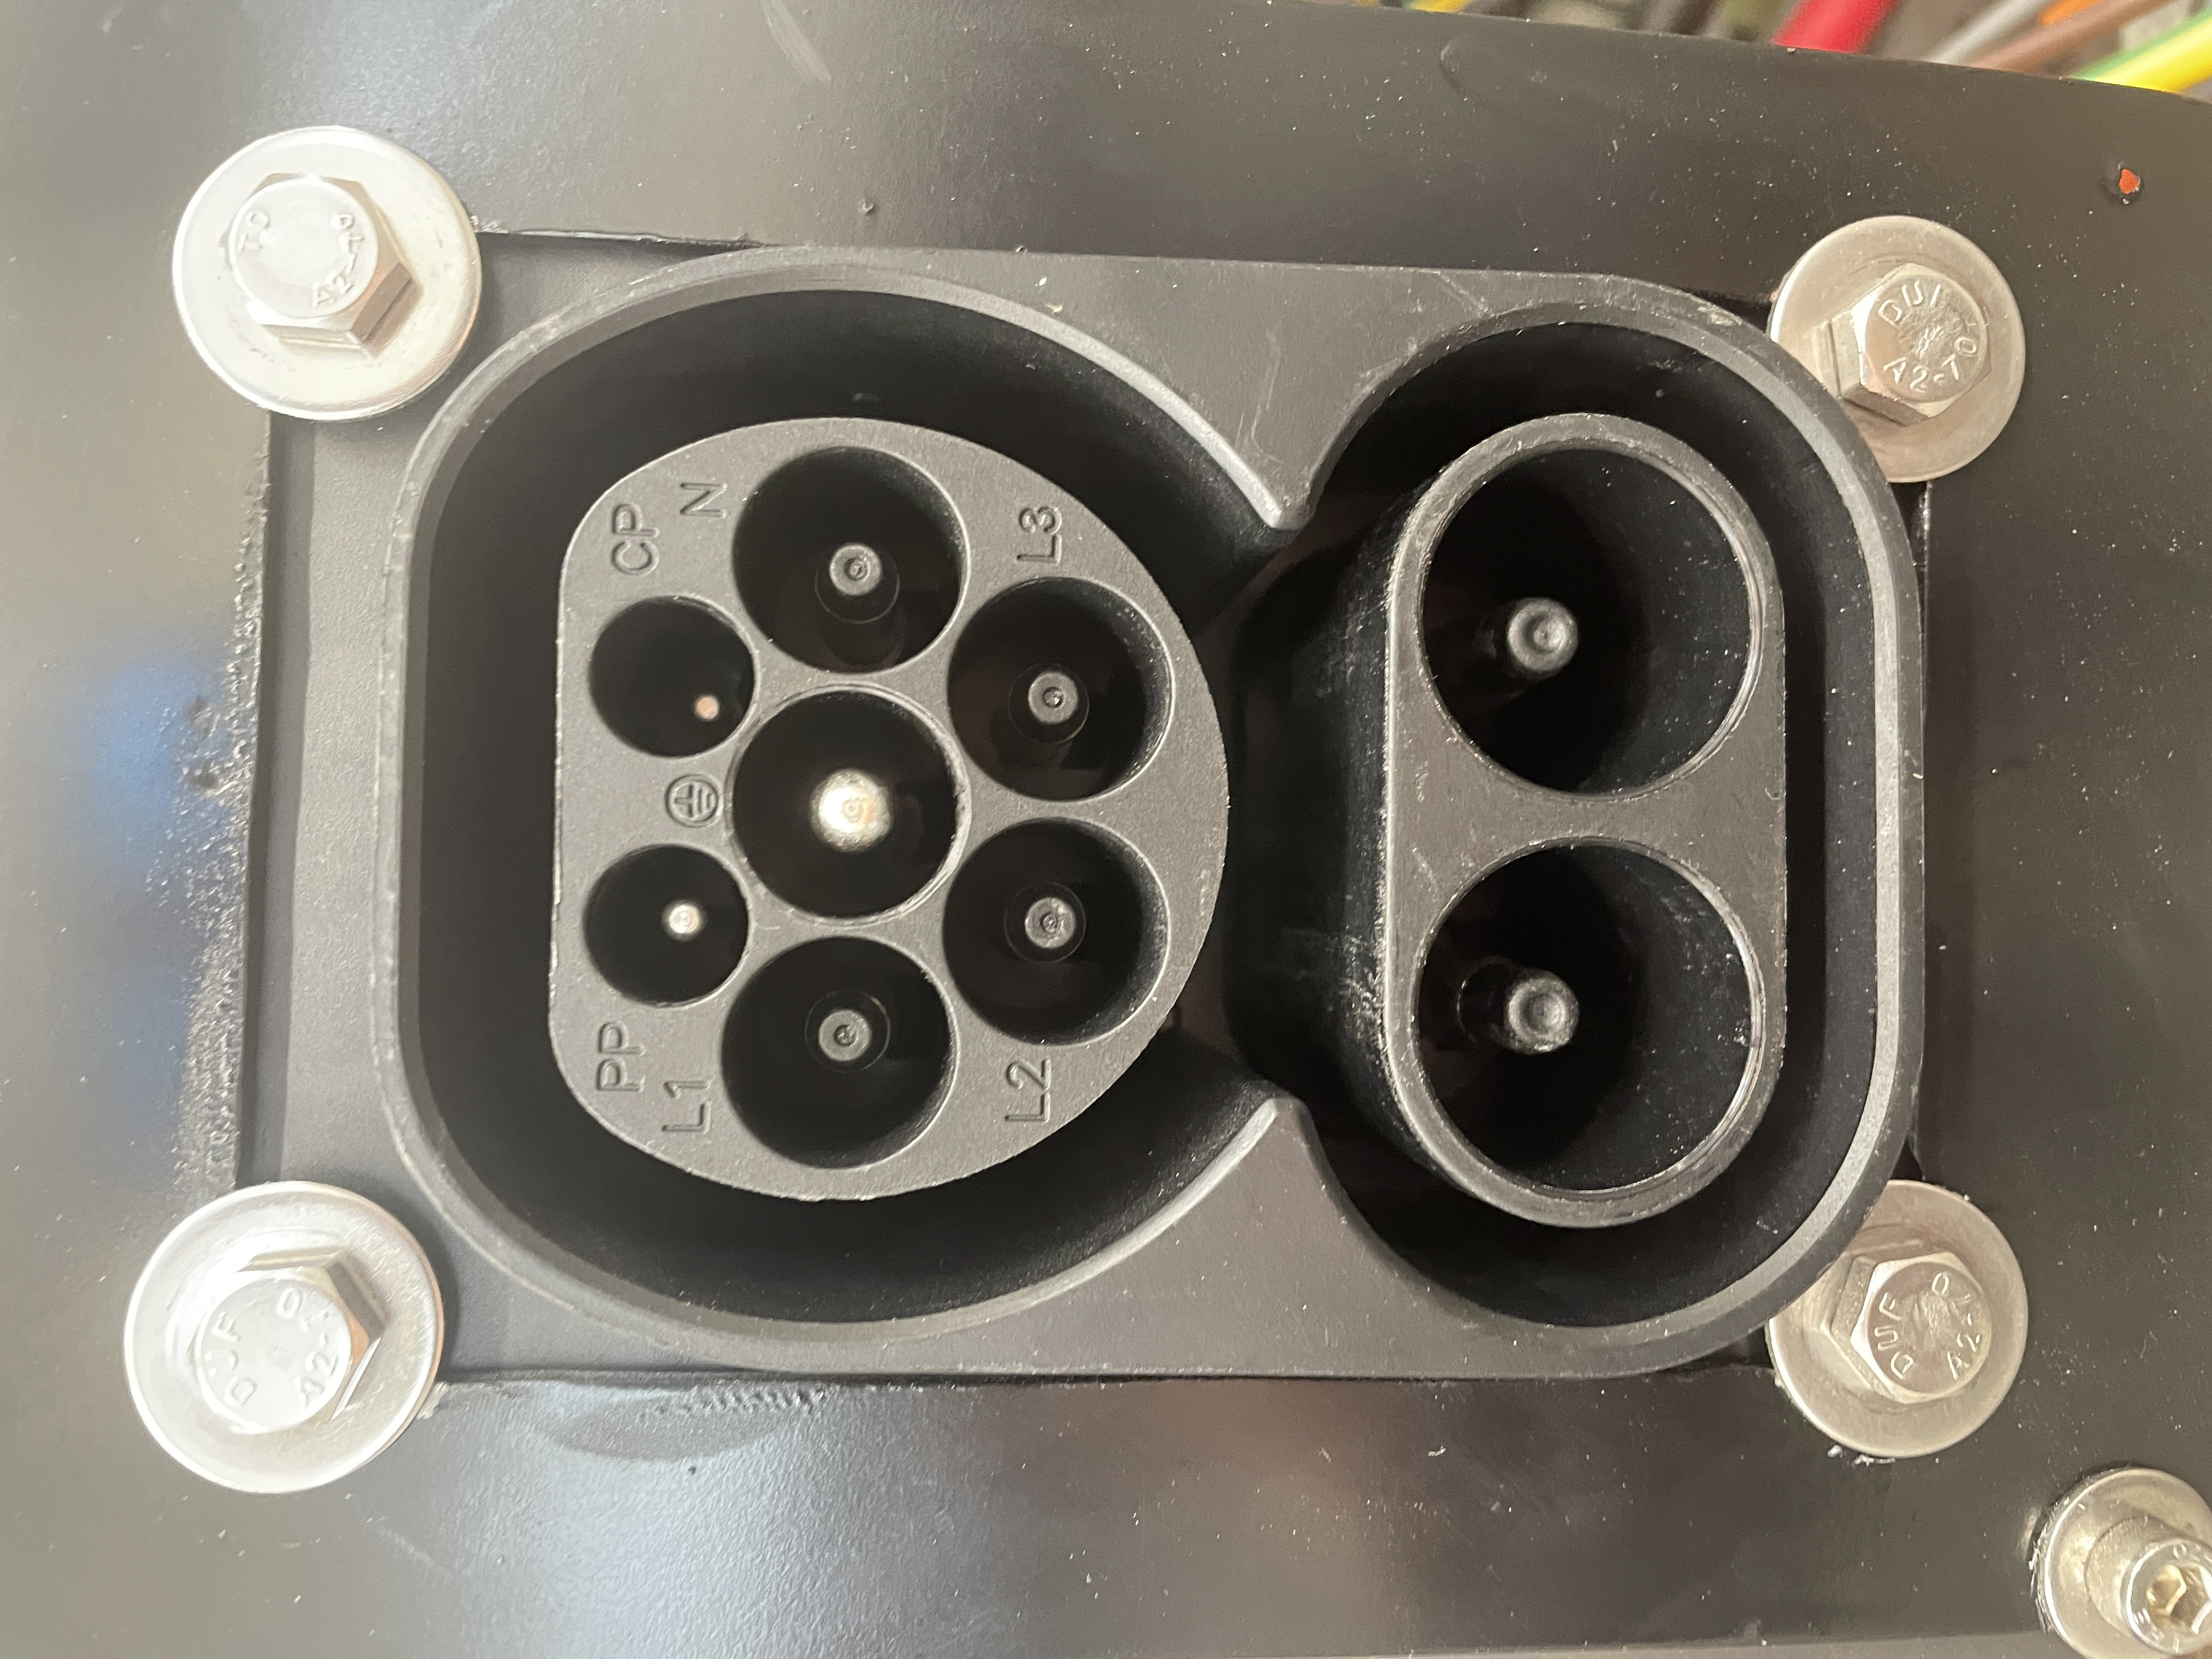
\includegraphics[width=0.9\textwidth,angle=-90]{CCS_combo2_inlet}}
        \caption{CCS Combo 2 inlet}
        \label{fig:CCS_combo2_inlet}
        \hfill
        \centerline{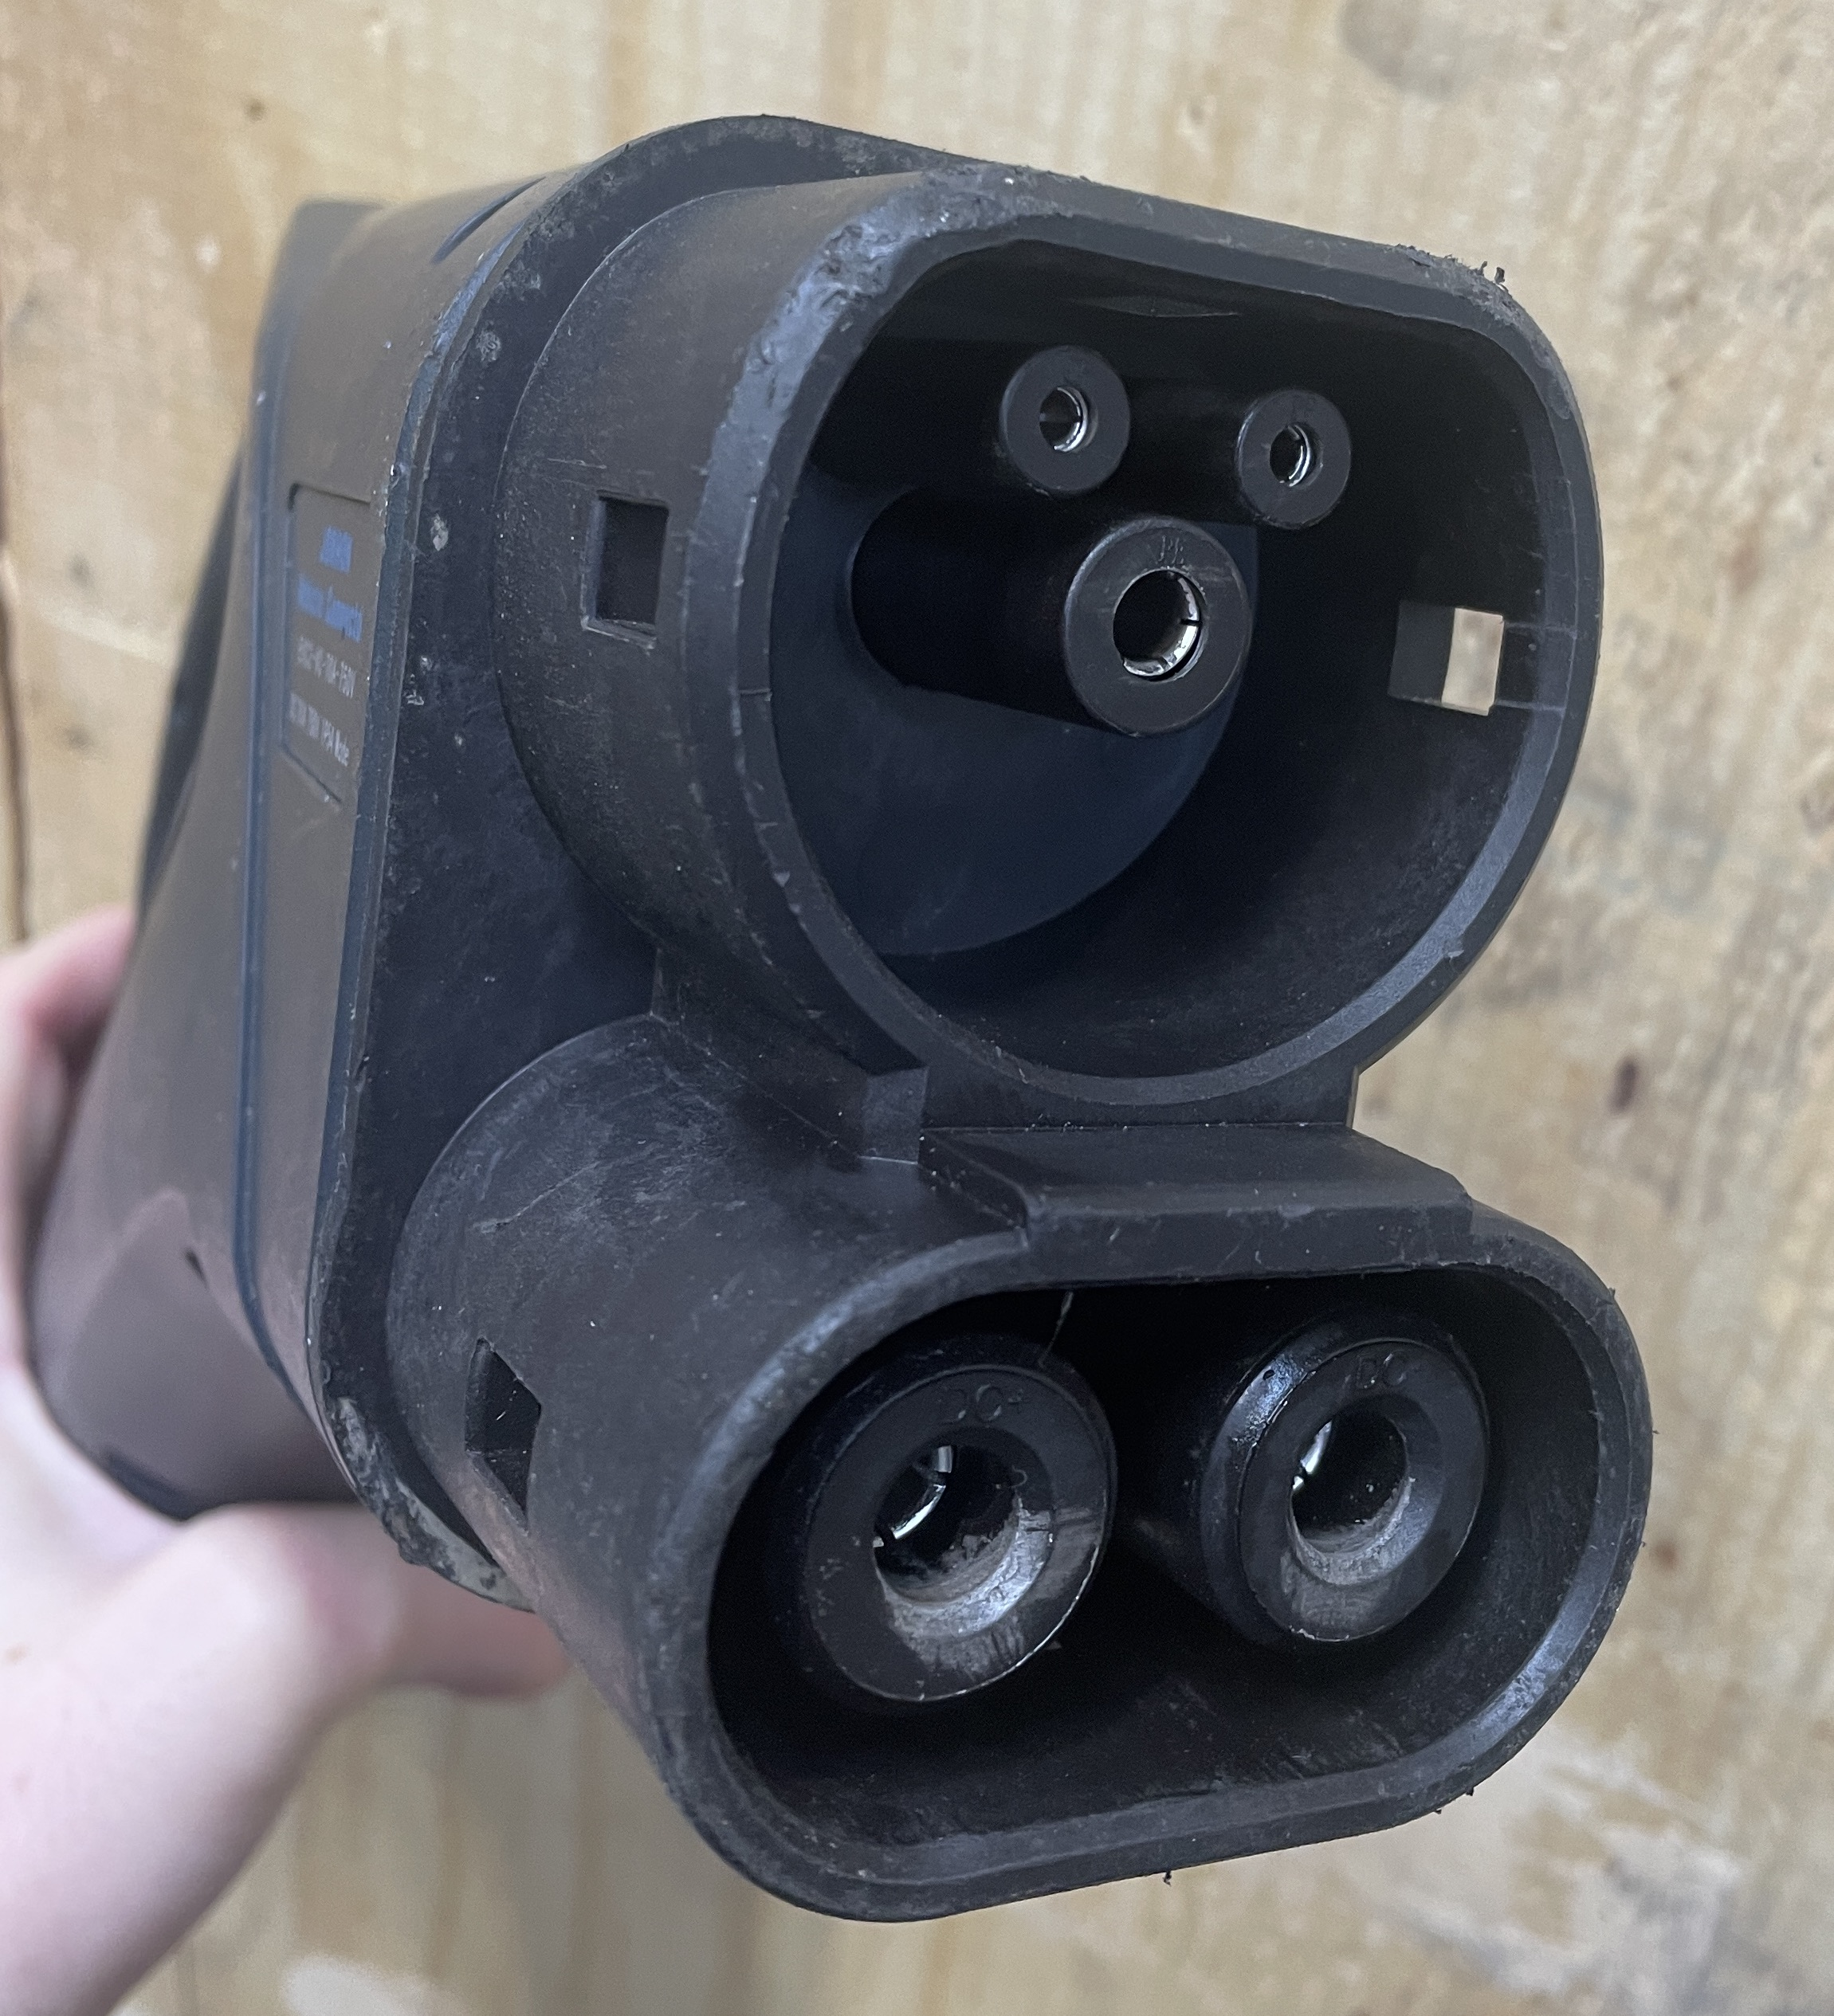
\includegraphics[width=0.9\textwidth]{CCS_combo2_outlet}}
        \caption{CCS Combo 2 outlet (stekker)}
        \label{fig:CCS_combo2_outlet}
    \end{minipage}
\end{figure}

%%%%%%%%%%%%%%%%%%%%%%%%%%%%%%%%%%%%%%%%%%%%%%%%%%%%%%%%%%%%%%%%%%%%%%%%
\subsubsection{AC laadden}
%%%%%%%%%%%%%%%%%%%%%%%%%%%%%%%%%%%%%%%%%%%%%%%%%%%%%%%%%%%%%%%%%%%%%%%%

\ac{ac} laaden kan ook nog op verschillende manieren en snelheden, het grootste
verschil is een phase en drie phase, waarbij 3 phase in princiepe drie keer
zosnel laad als een phase. Deze laadmethode gebruikt een interne laader in de
auto (\ac{ev}). En de comumicatie tussen de auto en de \ac{evse} is heel simpel
met een \ac{pwm} signal. Het \ac{pwm} signal word gebruikt om de maximale
stroom die de \ac{evse} kan leveren te comuniceren aan de \ac{ev}. De \ac{ev}
geeft dan het signal de \ac{ev} klaar is om te laaden en de \ac{evse} zet dan
netspanning op de poolen van de type 2 stekker (outlet).

%%%%%%%%%%%%%%%%%%%%%%%%%%%%%%%%%%%%%%%%%%%%%%%%%%%%%%%%%%%%%%%%%%%%%%%%
\subsubsection{DC laadden}
%%%%%%%%%%%%%%%%%%%%%%%%%%%%%%%%%%%%%%%%%%%%%%%%%%%%%%%%%%%%%%%%%%%%%%%%

\ac{dc} laaden word dus CCS laaden genoemd. De \ac{evse} gebruikt de Combo 2
outlet (stekker) en de \ac{ev} gebruikt de Combo 2 inlet (inlet). de \ac{evse}
is bij de laaden de laader, en wordt doormiddel van cantactoren in de \ac{ev}
dircet aan de accupolen aangeslooten. hiermee kan met veel hogere stroom woorde
gelaaden en daarom word \ac{dc} laaden ook wel snelladen genoemd.

\mainmatter

\chapter{Analyse van het probleem}
\label{Analyse_van_het_probleem}
%%%%%%%%%%%%%%%%%%%%%%%%%%%%%%%%%%%%%%%%%%%%%%%%%%%%%%%%%%%%%%%%%%%%%%%%

\begin{center}
    \begin{minipage}{0.5\textwidth}
        \begin{small}
            Waar de noodzaak van dit project word blootgelegd.
        \end{small} 
    \end{minipage}
    \vspace{0.5cm}
\end{center}

Kortweg is het probleem dat er momenteel niet met \ac{hdpe} en \ac{pp} kan
woorden ge-3D-print. 3D-printen met \ac{hdpe} en \ac{pp} is wenselijk omdat deze
materialen overvloedig zijn is de huidige afvalstroom, en ze dus goedkoop
te verkrijgen zijn.\\

Een voorbeeld van hoogwaardig PP in de afvalstroom zijn verpakkingen van
medische goederen in ziekenhuizen.  3devo heeft \ac{pp} bakjes van een
oogheelkunde kliniek en wil dat recyclen tot 3D-printer filament. Zie Figuur
\ref{fig:pp_bakjes} voor de bakjes.

\begin{figure}[h]
    \centerline{\includegraphics[width=0.4\textwidth]{pp_bakjes}}
    \caption{\ac{pp} bakjes van een oogheelkunde kliniek}
    \label{fig:pp_bakjes}
\end{figure}

%%%%%%%%%%%%%%%%%%%%%%%%%%%%%%%%%%%%%%%%%%%%%%%%%%%%%%%%%%%%%%%%%%%%%%%%
\section{Waarom is een speciale 3D-printer nodig}
%%%%%%%%%%%%%%%%%%%%%%%%%%%%%%%%%%%%%%%%%%%%%%%%%%%%%%%%%%%%%%%%%%%%%%%%

Er zijn twee redenen gegeven waarom een speciale printer nodig is voor het
printen met \ac{hdpe} en \ac{pp}.  Tests zijn uitgevoerd om vast te stellen of
deze complicaties werkelijk het printen van \ac{hdpe} en \ac{pp} onmogelijk
maken.

%%%%%%%%%%%%%%%%%%%%%%%%%%%%%%%%%%%%%%%%%%%%%%%%%%%%%%%%%%%%%%%%%%%%%%%%
\subsection{Printen op een conventionele 3D-printer}
%%%%%%%%%%%%%%%%%%%%%%%%%%%%%%%%%%%%%%%%%%%%%%%%%%%%%%%%%%%%%%%%%%%%%%%%

Er is een test uitgevoerd met het printen van \ac{hdpe} en \ac{pp}.  Deze test
zijn uitgevoerd op een conventionele \ac{fdm} 3D-printer, namelijk een Ender-3.
De slicer settings die gebruikt zijn waren vooral getweakt op temperatuur en
snelheid.

\begin{figure}[h]
    \centering
    \begin{minipage}{0.45\textwidth}
        \centerline{\includegraphics[width=0.9\textwidth]{hdpe_per_test}}
        \caption{Test print met \ac{hdpe} op een conventionele printer}
        \label{fig:hdpe_test}
    \end{minipage}\hfill
    \begin{minipage}{0.45\textwidth}
        \centerline{\includegraphics[width=0.9\textwidth]{pp_pre_test}}
        \caption{Test print met \ac{pp} op een conventionele printer}
        \label{fig:pp_test}
    \end{minipage}
\end{figure}

%%%%%%%%%%%%%%%%%%%%%%%%%%%%%%%%%%%%%%%%%%%%%%%%%%%%%%%%%%%%%%%%%%%%%%%%
\subsubsection{Laag hechting}
%%%%%%%%%%%%%%%%%%%%%%%%%%%%%%%%%%%%%%%%%%%%%%%%%%%%%%%%%%%%%%%%%%%%%%%%

De hypothese is dat bij het printen met \ac{pp} de laag hechting niet goed zal
zijn. Dat komt doordat \ac{pp} onder de kristallisatietemperatuur niet
''plakkerig'' is. De test met het printen van \ac{pp} heeft geconcludeerd dat
die hypothese waar is. Het materiaal blijft moeilijk plakken aan het bed, en als
dat goed ging, blijft het ook nauwelijks plakken aan zichzelf. Zie Figuur
\ref{fig:pp_test}. Een ander probleem met het printen van \ac{pp} is dat het
flexibele plastic niet goed door een bowden extruder gaat vanwege de extra
weerstand in dat systeem. Uitleg over wat een bowden tube extruder is staat in
hoofdstuk \ref{ss:Bowden_extruder}.

%%%%%%%%%%%%%%%%%%%%%%%%%%%%%%%%%%%%%%%%%%%%%%%%%%%%%%%%%%%%%%%%%%%%%%%%
\subsubsection{Krom trekken}
%%%%%%%%%%%%%%%%%%%%%%%%%%%%%%%%%%%%%%%%%%%%%%%%%%%%%%%%%%%%%%%%%%%%%%%%

De verwachting was dat het grote probleem met HDPE is dat het krom trekt tijdens
het printen. Tijdens het printen zal er een warmte gradiënt ontstaan, omdat de
laag die net is neergelegd al aan het afkoelen is voor dat de volgende de
volgende laag daar op word gelegd. Tijdens het testen op een conventionele
printer is vastgesteld dat dat inderdaad een probleem is, zie Figuur
\ref{fig:hdpe_test} voor een foto van de krom getrokken prints.

\chapter{Eisen van het project}
\label{Eisen_van_het_project}
%%%%%%%%%%%%%%%%%%%%%%%%%%%%%%%%%%%%%%%%%%%%%%%%%%%%%%%%%%%%%%%%%%%%%%%%

Er zijn eisen waar het project en product aan moet voldoen. Deze eisen zijn
onderverdeeld in dit hoofdstuk.

%%%%%%%%%%%%%%%%%%%%%%%%%%%%%%%%%%%%%%%%%%%%%%%%%%%%%%%%%%%%%%%%%%%%%%%%
\section{Randvoorwaarden}
% waar moet je je aan houden (en kan je vanuit het project niet veranderen)?
% Voorbeeld: wet- en regelgeving. De voorschriften van de accountant etc.
%%%%%%%%%%%%%%%%%%%%%%%%%%%%%%%%%%%%%%%%%%%%%%%%%%%%%%%%%%%%%%%%%%%%%%%%

Het modem en de CCS electronica moet communiceren met het BMS om de laadstroom en
de accuspanning aan de \ac{evse} te communiceren.

%%%%%%%%%%%%%%%%%%%%%%%%%%%%%%%%%%%%%%%%%%%%%%%%%%%%%%%%%%%%%%%%%%%%%%%%
\section{Functionele wensen}
% wat moet het resultaat kunnen/doen?
% Voorbeeld: 10.000 liter per uur zuiveren; 2500 broden per dag bakken;
% 500 aankopen per uur kunnen verwerken etc.
%%%%%%%%%%%%%%%%%%%%%%%%%%%%%%%%%%%%%%%%%%%%%%%%%%%%%%%%%%%%%%%%%%%%%%%%

Het uiteindelijk gewenste resultaat is een systeem dat in een elektrische auto
kan worden ingebouwd, waarmee de auto het CCS protocol volledig ondersteund. En
dus met \si{350\kilo\watt} kan laden als het accupakket dat ook aankan, en
anders met het maximale vermogen dat het accupakket aan kan.

%%%%%%%%%%%%%%%%%%%%%%%%%%%%%%%%%%%%%%%%%%%%%%%%%%%%%%%%%%%%%%%%%%%%%%%%
\section{Gebruikerswensen}
% welke eisen stellen gebruikers aan het resultaat?
% Voorbeeld: gebruikers moeten maximaal 3 keer doorklikken op de website om bij
% de informatie te komen die ze zoeken
%%%%%%%%%%%%%%%%%%%%%%%%%%%%%%%%%%%%%%%%%%%%%%%%%%%%%%%%%%%%%%%%%%%%%%%%

Het moet getest zijn en werken met alle CCS laadsysteemen die we langs de
snelweg tegen komen. Het moet makkelijk te gebruiken zijn en zo min mogelijk
handelingen vereisen van de gebruiker.

%%%%%%%%%%%%%%%%%%%%%%%%%%%%%%%%%%%%%%%%%%%%%%%%%%%%%%%%%%%%%%%%%%%%%%%%
\section{Ontwerpbeperkingen}
% eisen die te maken hebben met de bouw/constructie
% Voorbeeld: promotiefilmpje op Youtube mag maximaal 10 minuten lang zijn
%%%%%%%%%%%%%%%%%%%%%%%%%%%%%%%%%%%%%%%%%%%%%%%%%%%%%%%%%%%%%%%%%%%%%%%%

Het ontwerp moet voeldoen aan de eisen en regelgeving resteld door de \ac{rdw}.
Dit betekent dat het elektrish veilig en geisoleerd moet zijn, en dat alles
tegen de omgeving in en onder een auto kan (water- en stofdicht).

%%%%%%%%%%%%%%%%%%%%%%%%%%%%%%%%%%%%%%%%%%%%%%%%%%%%%%%%%%%%%%%%%%%%%%%%
\section{Eindproduct}
%%%%%%%%%%%%%%%%%%%%%%%%%%%%%%%%%%%%%%%%%%%%%%%%%%%%%%%%%%%%%%%%%%%%%%%%

Het eindproduct dient een systeem te zijn dat klanten van EV Europe, en EV
Europe zelf, in kunnen bouwen in geschikte auto's. Er moet dus makkelijk mee te
werken zijn en makkelijk te instaleren zijn. Het moet ook voldoen aan de
bovenstaande eisen.

\chapter{Problemen}
\label{Problemen}
%%%%%%%%%%%%%%%%%%%%%%%%%%%%%%%%%%%%%%%%%%%%%%%%%%%%%%%%%%%%%%%%%%%%%%%%

Tijdens het project zijn eer paar problemen opgetreden. Dezen hadden allemaal
te maken met de extruder en dat daar geen plastic meer uit komt (vast liep).

%%%%%%%%%%%%%%%%%%%%%%%%%%%%%%%%%%%%%%%%%%%%%%%%%%%%%%%%%%%%%%%%%%%%%%%%
\section{Smeltend plastic in de extruder}
\label{s:smeltendplastic}
%%%%%%%%%%%%%%%%%%%%%%%%%%%%%%%%%%%%%%%%%%%%%%%%%%%%%%%%%%%%%%%%%%%%%%%%

Een probleem waar al vrij snel tegen aan werd geloopen is dat de extruder vast
liep door dat het plastic te vroeg smelten, met het gevolg er geen plastic meer uit de nozel kwam.
Dit gebeurde telkens rond de zelfde tijd na het starten van een print.

%%%%%%%%%%%%%%%%%%%%%%%%%%%%%%%%%%%%%%%%%%%%%%%%%%%%%%%%%%%%%%%%%%%%%%%%
\subsection{Oorzaak}
%%%%%%%%%%%%%%%%%%%%%%%%%%%%%%%%%%%%%%%%%%%%%%%%%%%%%%%%%%%%%%%%%%%%%%%%

Dit probleem was het resultaat van warme drive gears (extruder tandwielen).
Heat creep is een term voor het warmte gradiënt door de metalen onderdelen van
de extruder. De stappenmotor van de extruder en de heater cartridge van het
hotend produceren allebei warmte. Deze warmte geleid door de hele extruder
assemblage en komt dus ook bij de drive gears. Als daardoor het plastic ook
warm word smelt het in de extruder. En kan het dus niet meer door de nozel
woorden geperst.

%%%%%%%%%%%%%%%%%%%%%%%%%%%%%%%%%%%%%%%%%%%%%%%%%%%%%%%%%%%%%%%%%%%%%%%%
\section{Dubbelvouwend plastic in de extruder}
\label{s:Dubbelvouwend}
%%%%%%%%%%%%%%%%%%%%%%%%%%%%%%%%%%%%%%%%%%%%%%%%%%%%%%%%%%%%%%%%%%%%%%%%

Een probleem tijdens het testen met een PP print wat dat het plastic dubbel
vouwde in de ruimte tussen de extruder tandwielen en de glijder naar de
extruder. Dit is dus een ander probleem dan beschreven in hoofdstuk
\ref{s:smeltendplastic}, dit probleem treed eerder op en zelfs als de kamer
niet is verwarmd. Dit probleem treden ook op tijdens het testen van PP op een
normaale printer, echter om een andere reden.

%%%%%%%%%%%%%%%%%%%%%%%%%%%%%%%%%%%%%%%%%%%%%%%%%%%%%%%%%%%%%%%%%%%%%%%%
\subsection{Oorzaak}
%%%%%%%%%%%%%%%%%%%%%%%%%%%%%%%%%%%%%%%%%%%%%%%%%%%%%%%%%%%%%%%%%%%%%%%%

Dit komt doordat er genoeg ruimte is tussen de extruder tandwielen en het
extruder frame dat er filament tussen door past. En omdat PP veel flexibeler is
dan HDPE, gaat het makkelijk daar tussen zitten.

Dit probleem had een adere oorzaak bij het testen op een standaard ender-3. De
oorzaak was echter dat de extruder veel meer kracht zou moeten zetten omdat de
ender-3 een bowden extruder printer is. Uitleg over wat een bowden tube
extruder is staat in hoofdstuk \ref{ss:Bowden_extruder}.


%%%%%%%%%%%%%%%%%%%%%%%%%%%%%%%%%%%%%%%%%%%%%%%%%%%%%%%%%%%%%%%%%%%%%%%%
\section{Kamer temperatuur overshoot}
%%%%%%%%%%%%%%%%%%%%%%%%%%%%%%%%%%%%%%%%%%%%%%%%%%%%%%%%%%%%%%%%%%%%%%%%

De temperatuur van de verwarmde kamer schiet door het setpoint heen voordat het
stabiliseert of oscilleert rond de ingestelde waarden

%%%%%%%%%%%%%%%%%%%%%%%%%%%%%%%%%%%%%%%%%%%%%%%%%%%%%%%%%%%%%%%%%%%%%%%%
\subsection{Oorzaak}
%%%%%%%%%%%%%%%%%%%%%%%%%%%%%%%%%%%%%%%%%%%%%%%%%%%%%%%%%%%%%%%%%%%%%%%%

De massa van de thermistor is zo hoog dat het lang duurt om in evenwicht te
komen met de luchttemperatuur. Daarom loopt de gemeenten temperatuur dus
aanzienlijk achter op de werkelijke temperatuur. De werkelijke temperatuur is
geverifieerd door een thermokoppel naast de thermistor te hangen.
\chapter{Mogelijke oplossingen}
\label{Mogelijke_oplossingen}
%%%%%%%%%%%%%%%%%%%%%%%%%%%%%%%%%%%%%%%%%%%%%%%%%%%%%%%%%%%%%%%%%%%%%%%%

%%%%%%%%%%%%%%%%%%%%%%%%%%%%%%%%%%%%%%%%%%%%%%%%%%%%%%%%%%%%%%%%%%%%%%%%
\section{Extruder problemen}
%%%%%%%%%%%%%%%%%%%%%%%%%%%%%%%%%%%%%%%%%%%%%%%%%%%%%%%%%%%%%%%%%%%%%%%%

Het probleem van een vastlopende extruder kwam voor met een direct drive
extruder. Een oplossing die overwogen was, was het overstappen naar een andere
extruder architectuur.

%%%%%%%%%%%%%%%%%%%%%%%%%%%%%%%%%%%%%%%%%%%%%%%%%%%%%%%%%%%%%%%%%%%%%%%%
\subsection{Verschillende soorten extruders}
%%%%%%%%%%%%%%%%%%%%%%%%%%%%%%%%%%%%%%%%%%%%%%%%%%%%%%%%%%%%%%%%%%%%%%%%

\begin{figure}[h]
    \centerline{\includegraphics[width=0.85\textwidth]{Basic-diagram-of-FDM-3D-printer-extruder-a-Direct-extruder-b-Bowden-extruder}}
    \caption{Diagram van de twee soorten extruders die veel woorden gebruikt \cite{soorten_extruders}.}
    \label{fig:soorten_extruders}
\end{figure}

%%%%%%%%%%%%%%%%%%%%%%%%%%%%%%%%%%%%%%%%%%%%%%%%%%%%%%%%%%%%%%%%%%%%%%%%
\subsubsection{Bowden extruder}
\label{ss:Bowden_extruder}
%%%%%%%%%%%%%%%%%%%%%%%%%%%%%%%%%%%%%%%%%%%%%%%%%%%%%%%%%%%%%%%%%%%%%%%%

De rechter helft van Figuur \ref{fig:soorten_extruders} \cite{soorten_extruders}
is een diagram van een Bowden extruder. Hierbij is te zien dat \ac{extruder} los
is van de \ac{hotend}.

% uitleg

%%%%%%%%%%%%%%%%%%%%%%%%%%%%%%%%%%%%%%%%%%%%%%%%%%%%%%%%%%%%%%%%%%%%%%%%
\subsubsection{Direct drive extruder}
\label{ss:direct_drive_extruder}
%%%%%%%%%%%%%%%%%%%%%%%%%%%%%%%%%%%%%%%%%%%%%%%%%%%%%%%%%%%%%%%%%%%%%%%%

De linker helft van Figuur \ref{fig:soorten_extruders} \cite{soorten_extruders}
is een diagram van een direct drive extruder.

% uitleg

%%%%%%%%%%%%%%%%%%%%%%%%%%%%%%%%%%%%%%%%%%%%%%%%%%%%%%%%%%%%%%%%%%%%%%%%
\subsection{Zou een Bowden extruder de problemen oplossen}
%%%%%%%%%%%%%%%%%%%%%%%%%%%%%%%%%%%%%%%%%%%%%%%%%%%%%%%%%%%%%%%%%%%%%%%%

Met een bowden extruder zou het probleem van smeltend plastic in de extruder
(Hoofdstuk \ref{s:smeltendplastic}) opgelost kunnen woorden. Echter was
opgemerkt dat PP niet geprint kan woorden met een bowden printer (Hoofdstuk
\ref{s:Dubbelvouwend}).

%%%%%%%%%%%%%%%%%%%%%%%%%%%%%%%%%%%%%%%%%%%%%%%%%%%%%%%%%%%%%%%%%%%%%%%%
\subsection{Zou een water gekoelde extruder de problemen oplossen}
%%%%%%%%%%%%%%%%%%%%%%%%%%%%%%%%%%%%%%%%%%%%%%%%%%%%%%%%%%%%%%%%%%%%%%%%

Een water gekoelde extruder/hotend zou allebei de problemen kunnen oplossen met
als enige nadeel extra complexheid in de vorm van aanstuur elektronica en
software voor de waterkoeling en de waterkoeling zelf (buizen, pomp, radiator).

Een goede optie zou de "Titan Aqua" \cite{titanaqua} zijn.

% bronvermedling naar pagina over watergekoelde hotend/extruder

%%%%%%%%%%%%%%%%%%%%%%%%%%%%%%%%%%%%%%%%%%%%%%%%%%%%%%%%%%%%%%%%%%%%%%%%
\section{Temperatuur overshoot}
%%%%%%%%%%%%%%%%%%%%%%%%%%%%%%%%%%%%%%%%%%%%%%%%%%%%%%%%%%%%%%%%%%%%%%%%

Een \ac{PID} lus voor de kamertemperatuur kan woorden geïmplementeerd in de
firmware van de printer, het vermogen van de warmte-elementen kan worden
teruggedraaid om ervoor te zorgen dat de temperatuur minder snel stijgt en er
dus een minder groot verschil is tussen de gemeenten en de werkelijke
temperatuur.

\chapter{De gekozen oplossing}
\label{De_gekozen_oplossing}
%%%%%%%%%%%%%%%%%%%%%%%%%%%%%%%%%%%%%%%%%%%%%%%%%%%%%%%%%%%%%%%%%%%%%%%%

Om een keuze te maken tussen Advantics en Zero-EV zijn beide modems onderzocht,
en is de beste optie gekozen, in dit hoofdstuk word die keuze gemaakt en
uitgelicht.

%%%%%%%%%%%%%%%%%%%%%%%%%%%%%%%%%%%%%%%%%%%%%%%%%%%%%%%%%%%%%%%%%%%%%%%%
\section{Welk modem}
%%%%%%%%%%%%%%%%%%%%%%%%%%%%%%%%%%%%%%%%%%%%%%%%%%%%%%%%%%%%%%%%%%%%%%%%

Om een goede keuze te maken tussen Advantics en Zero-EV zijn beide modems
onderzocht door de datasheets om alle eigenschappen van deze modems te
bekijken. Daar zijn voordelen en nadelen uitgekomen voor beide modems.

%%%%%%%%%%%%%%%%%%%%%%%%%%%%%%%%%%%%%%%%%%%%%%%%%%%%%%%%%%%%%%%%%%%%%%%%
\subsection{Advantics}
%%%%%%%%%%%%%%%%%%%%%%%%%%%%%%%%%%%%%%%%%%%%%%%%%%%%%%%%%%%%%%%%%%%%%%%%

De eerste periode was besteed aan het kijken naar de mogelijkheden van het
Advantics systeem. In figuur \ref{fig:advantics_overzicht} zie je een overzicht
van alle componenten van het Advantics systeem. Centraal staat de \ac{ecu} met
geïntegreerd modem. Deze \ac{ecu} is ook gelijk de contactor controller (hij
kan de CCS-contractors in de EV aansturen).

\begin{figure}[h]
    \centering
    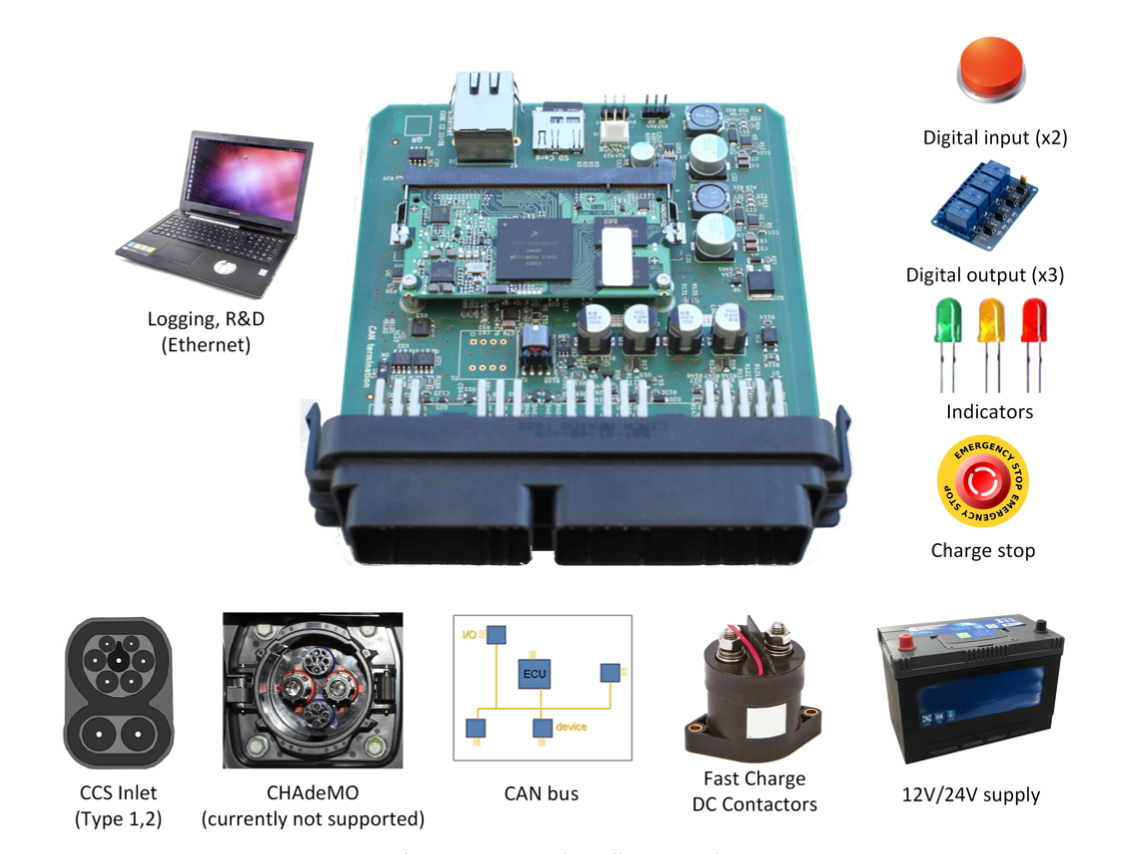
\includegraphics[width=0.85\textwidth]{advantics_overzicht}
    \caption{Overzicht van het Advantics systeem}
    \label{fig:advantics_overzicht}
\end{figure}

Waar al vrij snel tegen aan werd gelopen is dat de handleiding van dit systeem
incompleet is. Bovendien is de software die draait op de \ac{ecu} niet klaar om
te gebruiken. De fabrikant gaat ervan uit dat de gebruiker software schrijft
voor communicatie met het \ac{bms} en met de \ac{evse}. Maar het was niet
duidelijk hoe voor dit systeem ontwikkeld moest worden, als er geen/slechte
documentatie was.

\begin{table}[h]
    \begin{tabular}{|c|c|}
        \hline
        \multicolumn{2}{c}{Advantics} \\
        \hline
        Voordelen           & Nadelen \\
        \hline
        Heel erg uitgebreid & Moeilijk te gebruiken \\
        Veel mogelijkheden  & Er moet firmware voor ontwikkeld worden \\
        \hline
    \end{tabular}
\end{table}

%%%%%%%%%%%%%%%%%%%%%%%%%%%%%%%%%%%%%%%%%%%%%%%%%%%%%%%%%%%%%%%%%%%%%%%%
\subsection{Zero-EV}
%%%%%%%%%%%%%%%%%%%%%%%%%%%%%%%%%%%%%%%%%%%%%%%%%%%%%%%%%%%%%%%%%%%%%%%%

Hey systeem van Zero-EV zit iets anders in elkaar. Het systeem bestaat uit een
\ac{ecu} met een intern modem en een CCS contactor controller. Die onderdelen
communiceren met het BMS over de \ac{can} bus. In figuur
\ref{fig:zeroev_overzicht} zie je een overzicht van alle componenten van het
systeem.

\begin{figure}[h]
    \centering
    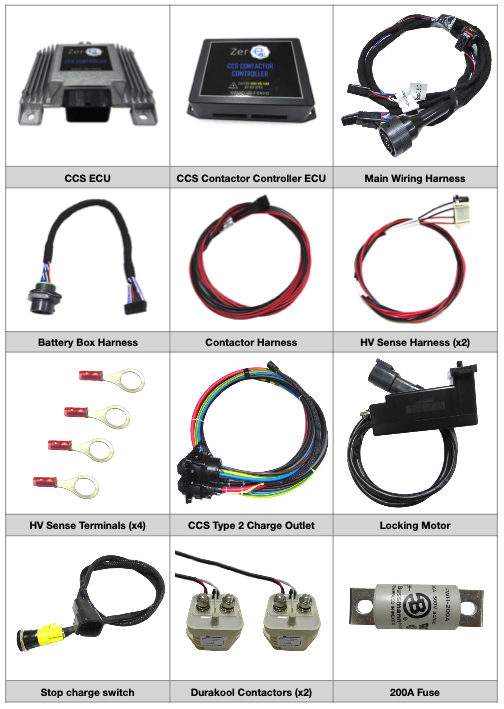
\includegraphics[width=0.45\textwidth]{zeroev_overzicht}
    \caption{Overzicht van het Zero-EV systeem}
    \label{fig:zeroev_overzicht}
\end{figure}

Het systeem van Zero-EV zou plug-and-play moeten zijn. Echter is dat alleen zo
als je een Orion BMS gebruikt, en EV Europe werkt met het EMUS BMS-systeem.

Als voor dit systeem wordt gekozen moet dus iets worden ontworpen dat er voor
zorgt dat het werkt met EMUS \ac{bms}.

\begin{table}[h]
    \begin{tabular}{|c|c|}
        \hline
        \multicolumn{2}{c}{Zero-EV} \\
        \hline
        Voordelen                          & Nadelen \\
        \hline
        Plug-and-play (met het juiste BMS) & Niet door de gebruiker te configureren \\
        Goede documentatie                 & \\
        \hline
    \end{tabular}
\end{table}

%%%%%%%%%%%%%%%%%%%%%%%%%%%%%%%%%%%%%%%%%%%%%%%%%%%%%%%%%%%%%%%%%%%%%%%%
\section{Conclusie}
%%%%%%%%%%%%%%%%%%%%%%%%%%%%%%%%%%%%%%%%%%%%%%%%%%%%%%%%%%%%%%%%%%%%%%%%

Na tijd te hebben besteed aan beiden systemen, is in overleg met de
opdrachtgever er voor gekozen om verder te gaan met het systeem van Zero-EV.
Deze keuze is gebaseerd op de voordelen en nadelen van beide modems, en hoe
realistisch het is dat het systeem op tijd af is (binnen de stageperiode).

\chapter{Ontwerp van de oplossing en de benodigde onderdelen}
\label{Ontwerp_van_de_oplossing_en_de_benodigde_onderdelen}
%%%%%%%%%%%%%%%%%%%%%%%%%%%%%%%%%%%%%%%%%%%%%%%%%%%%%%%%%%%%%%%%%%%%%%%%

Uit het vooronderzoek is het Zero-EV modem gekozen (Zie hoofdstuk
\ref{De_gekozen_oplossing}). En er is bepaald dat er een oplossing nodig is om
dat modem samen te laten werken met het BMS van EMUS. De communicatie van het
BMS en van het modem is volgens het CAN-protocol. Dus er moet een manier worden
verzonnen om de juiste CAN berichten naar het modem te sturen.

%%%%%%%%%%%%%%%%%%%%%%%%%%%%%%%%%%%%%%%%%%%%%%%%%%%%%%%%%%%%%%%%%%%%%%%%
\section{Can berichten}
%%%%%%%%%%%%%%%%%%%%%%%%%%%%%%%%%%%%%%%%%%%%%%%%%%%%%%%%%%%%%%%%%%%%%%%%

De CAN-bus is een robuuste standaard waarmee microcontrollers in een auto data
kunnen uitwisselen. Die data word gestuurd in de vorm van berichten op de CAN
bus. Zo'n bericht heeft een CAN ID, wat aangeeft wat voor data het is, een
lengte en de data in het bericht zelf. Na contact te hebben gehad met Zero-EV,
hebben ze het \ac{dbc} bestand opgestuurd. Dit bestand kan worden gebruikt om
de CAN berichten te decoderen. Hierin staat informatie als: welk apparaat die
berichten genereert, voor welken apparaten die berichten bedoeld zijn, welken
bits en bytes in het CAN bericht welken data bevatten en de schaal en eenheid
van die data. \cite{DBC_File_Database_Intro}

%%%%%%%%%%%%%%%%%%%%%%%%%%%%%%%%%%%%%%%%%%%%%%%%%%%%%%%%%%%%%%%%%%%%%%%%
\subsection{Welken berichten moeten verstuurd worden}
%%%%%%%%%%%%%%%%%%%%%%%%%%%%%%%%%%%%%%%%%%%%%%%%%%%%%%%%%%%%%%%%%%%%%%%%

Voor het doeleinde van het project is dit DBC-bestand gebruikt om de juiste CAN
berichten te genereren voor het CCS-modem. Door uit dat bestand te herleiden
welken berichten het CCS-modem verwacht te ontvangen, en wat er in die
berichten moet staan.

%%%%%%%%%%%%%%%%%%%%%%%%%%%%%%%%%%%%%%%%%%%%%%%%%%%%%%%%%%%%%%%%%%%%%%%%
\subsubsection{Test data}
%%%%%%%%%%%%%%%%%%%%%%%%%%%%%%%%%%%%%%%%%%%%%%%%%%%%%%%%%%%%%%%%%%%%%%%%

Initieel tijdens de proof of consept fasen van dit idee stuurden we gewoon test
data naar het CCS-modem. Dat betekent dat we data stuurden in de CAN berichten,
zoals de accu spanning, die met de hand waren gemeten. Dit is echter niet hoe
het uiteindelijke product dient te functioneren. Er moet namelijk naar de CAN
bus van het BMS worden geluisterd om de juiste data te ontvangen.

%%%%%%%%%%%%%%%%%%%%%%%%%%%%%%%%%%%%%%%%%%%%%%%%%%%%%%%%%%%%%%%%%%%%%%%%
\subsubsection{Uiteindelijke data}
%%%%%%%%%%%%%%%%%%%%%%%%%%%%%%%%%%%%%%%%%%%%%%%%%%%%%%%%%%%%%%%%%%%%%%%%

De CAN bericht die het BMS verstuurd zijn beschreven in een handleiding van het
BMS, en toen ontdekt was wat het format daarvan is, kon het BMS worden
uitgelezen. Deze data kan dan worden vertaal naar CAN-berichten die het CCS
modem begrijpt.

%%%%%%%%%%%%%%%%%%%%%%%%%%%%%%%%%%%%%%%%%%%%%%%%%%%%%%%%%%%%%%%%%%%%%%%%
\section{Electronica}
%%%%%%%%%%%%%%%%%%%%%%%%%%%%%%%%%%%%%%%%%%%%%%%%%%%%%%%%%%%%%%%%%%%%%%%%

Voor de elektronica is dus een microcontroller nodig die over de CAN-bus
communiceren. Er is voor een microcontroller gekozen die compatibel is met de
Arduino \ac{ide}. En daarmee dus met C++ kan worden geprogrammeerd. Hier is
voor gekozen omdat hiermee makkelijk te werken is er dus meer tijd kan worden
besteed aan het ontwerpen en schrijven van de firmware, en minder aan het
instellen en debuggen van de editor/IDE.

Voor de CAN-interface van de microcontroller is een MCP2515 module gekozen
omdat dezen goed verkrijgbaar en goedkoop zijn en ook deze module goed kan
communiceren met de CAN-bus en de Arduino. \cite{canbord}

%%%%%%%%%%%%%%%%%%%%%%%%%%%%%%%%%%%%%%%%%%%%%%%%%%%%%%%%%%%%%%%%%%%%%%%%
\section{Software}
%%%%%%%%%%%%%%%%%%%%%%%%%%%%%%%%%%%%%%%%%%%%%%%%%%%%%%%%%%%%%%%%%%%%%%%%

Deze module communiceert over via de \ac{spi} met de microcontroller. Om de
communicatie makkelijker en de code overzichtelijker te maken is een
bibliotheek van autowp gebruikt \cite{autowp} samen met de standaard SPI
bibliotheek van Arduino gebruikt. Het fijne van deze bibliotheek is dat je de
bits en bytes van de CAN-berichten helemaal zelf kan manipuleren, om zo de
gewenste berichten te krijgen. Een kopie van de firmware is te vinden in
bijlagen \ref{code}.

%%%%%%%%%%%%%%%%%%%%%%%%%%%%%%%%%%%%%%%%%%%%%%%%%%%%%%%%%%%%%%%%%%%%%%%%
\section{Prototype}
%%%%%%%%%%%%%%%%%%%%%%%%%%%%%%%%%%%%%%%%%%%%%%%%%%%%%%%%%%%%%%%%%%%%%%%%

Voordat de uiteindelijke versie is gemaakt, zijn eerst alle onderdelen
tijdelijk aan elkaar gekopeld in een testopstelling. Pas toen werd
geconcludeerd dat de hardware van het prototypen werkt, is het in een behuizing
ingebouwd.

Wel zijn net andere componenten gebruikt, maar die zijn behlaven hun klijnere
formaat, voor deze doeleinde funktioneel identiek aan het prototype.

%%%%%%%%%%%%%%%%%%%%%%%%%%%%%%%%%%%%%%%%%%%%%%%%%%%%%%%%%%%%%%%%%%%%%%%%
\section{Proefopstelling}
\label{sec:proefopstelling}
%%%%%%%%%%%%%%%%%%%%%%%%%%%%%%%%%%%%%%%%%%%%%%%%%%%%%%%%%%%%%%%%%%%%%%%%

Het uiteidelijke product dient in een auto ingeboud en getest te worden, maar
omdat het niet handig is om te testen met een voledige auto, is er een
proefopstelling hebouwd. met alle onderdelen die nodig zijn om CCS werkend te
krijgen. zie figuur \ref{fig:proefopstelling} voor een afbeelding van de
proefopstelling.

\begin{figure}[]
    \centering
    \includegraphics[width=0.45\textwidth]{proefopstelling}
    \caption{Proefopstellig voor het CCS-modem}
    \label{fig:proefopstelling}
\end{figure}
\chapter{Assemblage}
\label{Assemblage}
%%%%%%%%%%%%%%%%%%%%%%%%%%%%%%%%%%%%%%%%%%%%%%%%%%%%%%%%%%%%%%%%%%%%%%%%

%%%%%%%%%%%%%%%%%%%%%%%%%%%%%%%%%%%%%%%%%%%%%%%%%%%%%%%%%%%%%%%%%%%%%%%%
\section{Assemblage van de printer}
%%%%%%%%%%%%%%%%%%%%%%%%%%%%%%%%%%%%%%%%%%%%%%%%%%%%%%%%%%%%%%%%%%%%%%%%

Het mechanisch ontwerp van de printer was al vastgesteld, de printer hoefde dus
alleen nog in elkaar woorden gezet. De printer is gebaseerd op de Ender-5, een
robuuste printer die een goed platform bied om een geïsoleerde behuizing  er
omheen te bouwen. De printer is voorzien van dubbele laser gesnelde wanden met
glas wol daar tussen. Ondank dat de assemblage van de behuizing niet in de
scoop van het project valt, was het wal nodig om verder te gaan met het
project. dus dat was als eerste gedaan.

%%%%%%%%%%%%%%%%%%%%%%%%%%%%%%%%%%%%%%%%%%%%%%%%%%%%%%%%%%%%%%%%%%%%%%%%
\subsection{Electronich}
%%%%%%%%%%%%%%%%%%%%%%%%%%%%%%%%%%%%%%%%%%%%%%%%%%%%%%%%%%%%%%%%%%%%%%%%

Electronich gezien moest er voral een hoop cable mangiment gebeuren. En de
firmware moest op het borad woorden gezet.

%%%%%%%%%%%%%%%%%%%%%%%%%%%%%%%%%%%%%%%%%%%%%%%%%%%%%%%%%%%%%%%%%%%%%%%%
% \section{Assemblage van de oplossing}
%%%%%%%%%%%%%%%%%%%%%%%%%%%%%%%%%%%%%%%%%%%%%%%%%%%%%%%%%%%%%%%%%%%%%%%%

%%%%%%%%%%%%%%%%%%%%%%%%%%%%%%%%%%%%%%%%%%%%%%%%%%%%%%%%%%%%%%%%%%%%%%%%
% \subsection{Subsection}
%%%%%%%%%%%%%%%%%%%%%%%%%%%%%%%%%%%%%%%%%%%%%%%%%%%%%%%%%%%%%%%%%%%%%%%%

% \chapter{Ondervonden problemen}
\label{Ondervonden_problemen}
%%%%%%%%%%%%%%%%%%%%%%%%%%%%%%%%%%%%%%%%%%%%%%%%%%%%%%%%%%%%%%%%%%%%%%%%

% drive gears overtemp
% heated chaimber to much overshoot (oplosing 1, verminder vermogen van heraters. oplosing 2 implementeer pid lus)
%
%

%%%%%%%%%%%%%%%%%%%%%%%%%%%%%%%%%%%%%%%%%%%%%%%%%%%%%%%%%%%%%%%%%%%%%%%%
%\section{Hardware}
%%%%%%%%%%%%%%%%%%%%%%%%%%%%%%%%%%%%%%%%%%%%%%%%%%%%%%%%%%%%%%%%%%%%%%%%

%%%%%%%%%%%%%%%%%%%%%%%%%%%%%%%%%%%%%%%%%%%%%%%%%%%%%%%%%%%%%%%%%%%%%%%%
%\section{Electronica}
%%%%%%%%%%%%%%%%%%%%%%%%%%%%%%%%%%%%%%%%%%%%%%%%%%%%%%%%%%%%%%%%%%%%%%%%

%%%%%%%%%%%%%%%%%%%%%%%%%%%%%%%%%%%%%%%%%%%%%%%%%%%%%%%%%%%%%%%%%%%%%%%%
%\section{Software}
%%%%%%%%%%%%%%%%%%%%%%%%%%%%%%%%%%%%%%%%%%%%%%%%%%%%%%%%%%%%%%%%%%%%%%%%


% \chapter{Eindresultaat}
\label{Eindresultaat}
%%%%%%%%%%%%%%%%%%%%%%%%%%%%%%%%%%%%%%%%%%%%%%%%%%%%%%%%%%%%%%%%%%%%%%%%

Het eindresultaat is een kleine behuizing met een Arduino Pro Mini, een MPC2515
module, een DC-DC converter als \ac{psu} en een generieke \ac{usb}-serial
(alleen nodig voor een Arduino Pro Mini) convertor.

Deze onderdelen zijn gekozen omdat ze makkelijk te verkrijgen en goedkoop
waren.

%%%%%%%%%%%%%%%%%%%%%%%%%%%%%%%%%%%%%%%%%%%%%%%%%%%%%%%%%%%%%%%%%%%%%%%%
\section{Schema}
%%%%%%%%%%%%%%%%%%%%%%%%%%%%%%%%%%%%%%%%%%%%%%%%%%%%%%%%%%%%%%%%%%%%%%%%

\begin{figure}[]
    \centering
    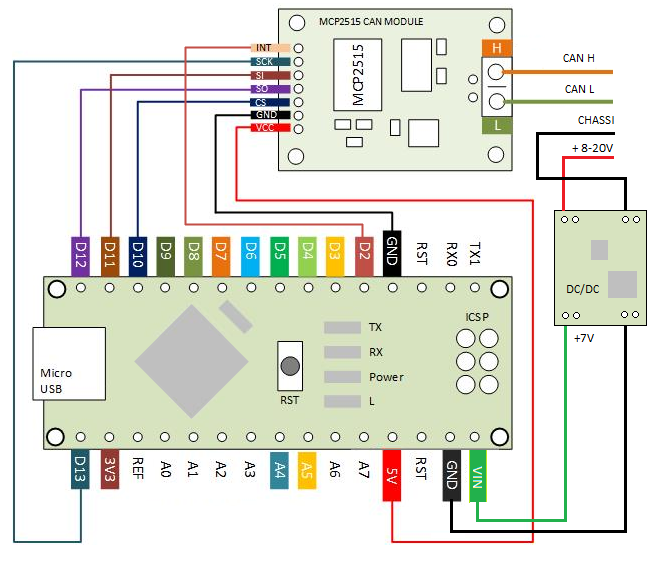
\includegraphics[width=0.45\textwidth]{wiring}
    \caption{Schema van de bedrading van de CAN-controller aan de Arduino \cite{autowp}}
    \label{fig:wiring}
\end{figure}

In het schema in figuur \ref{fig:wiring} is te zien hoe de Arduino de
CAN-controller aan kan sturen. En hoe de Arduino gevoed word met de
\si{12\volt} uit de auto.

%%%%%%%%%%%%%%%%%%%%%%%%%%%%%%%%%%%%%%%%%%%%%%%%%%%%%%%%%%%%%%%%%%%%%%%%
\section{Behuizing}
%%%%%%%%%%%%%%%%%%%%%%%%%%%%%%%%%%%%%%%%%%%%%%%%%%%%%%%%%%%%%%%%%%%%%%%%

\begin{figure}[]
    \centering
    \begin{minipage}{0.45\textwidth}
        \centerline{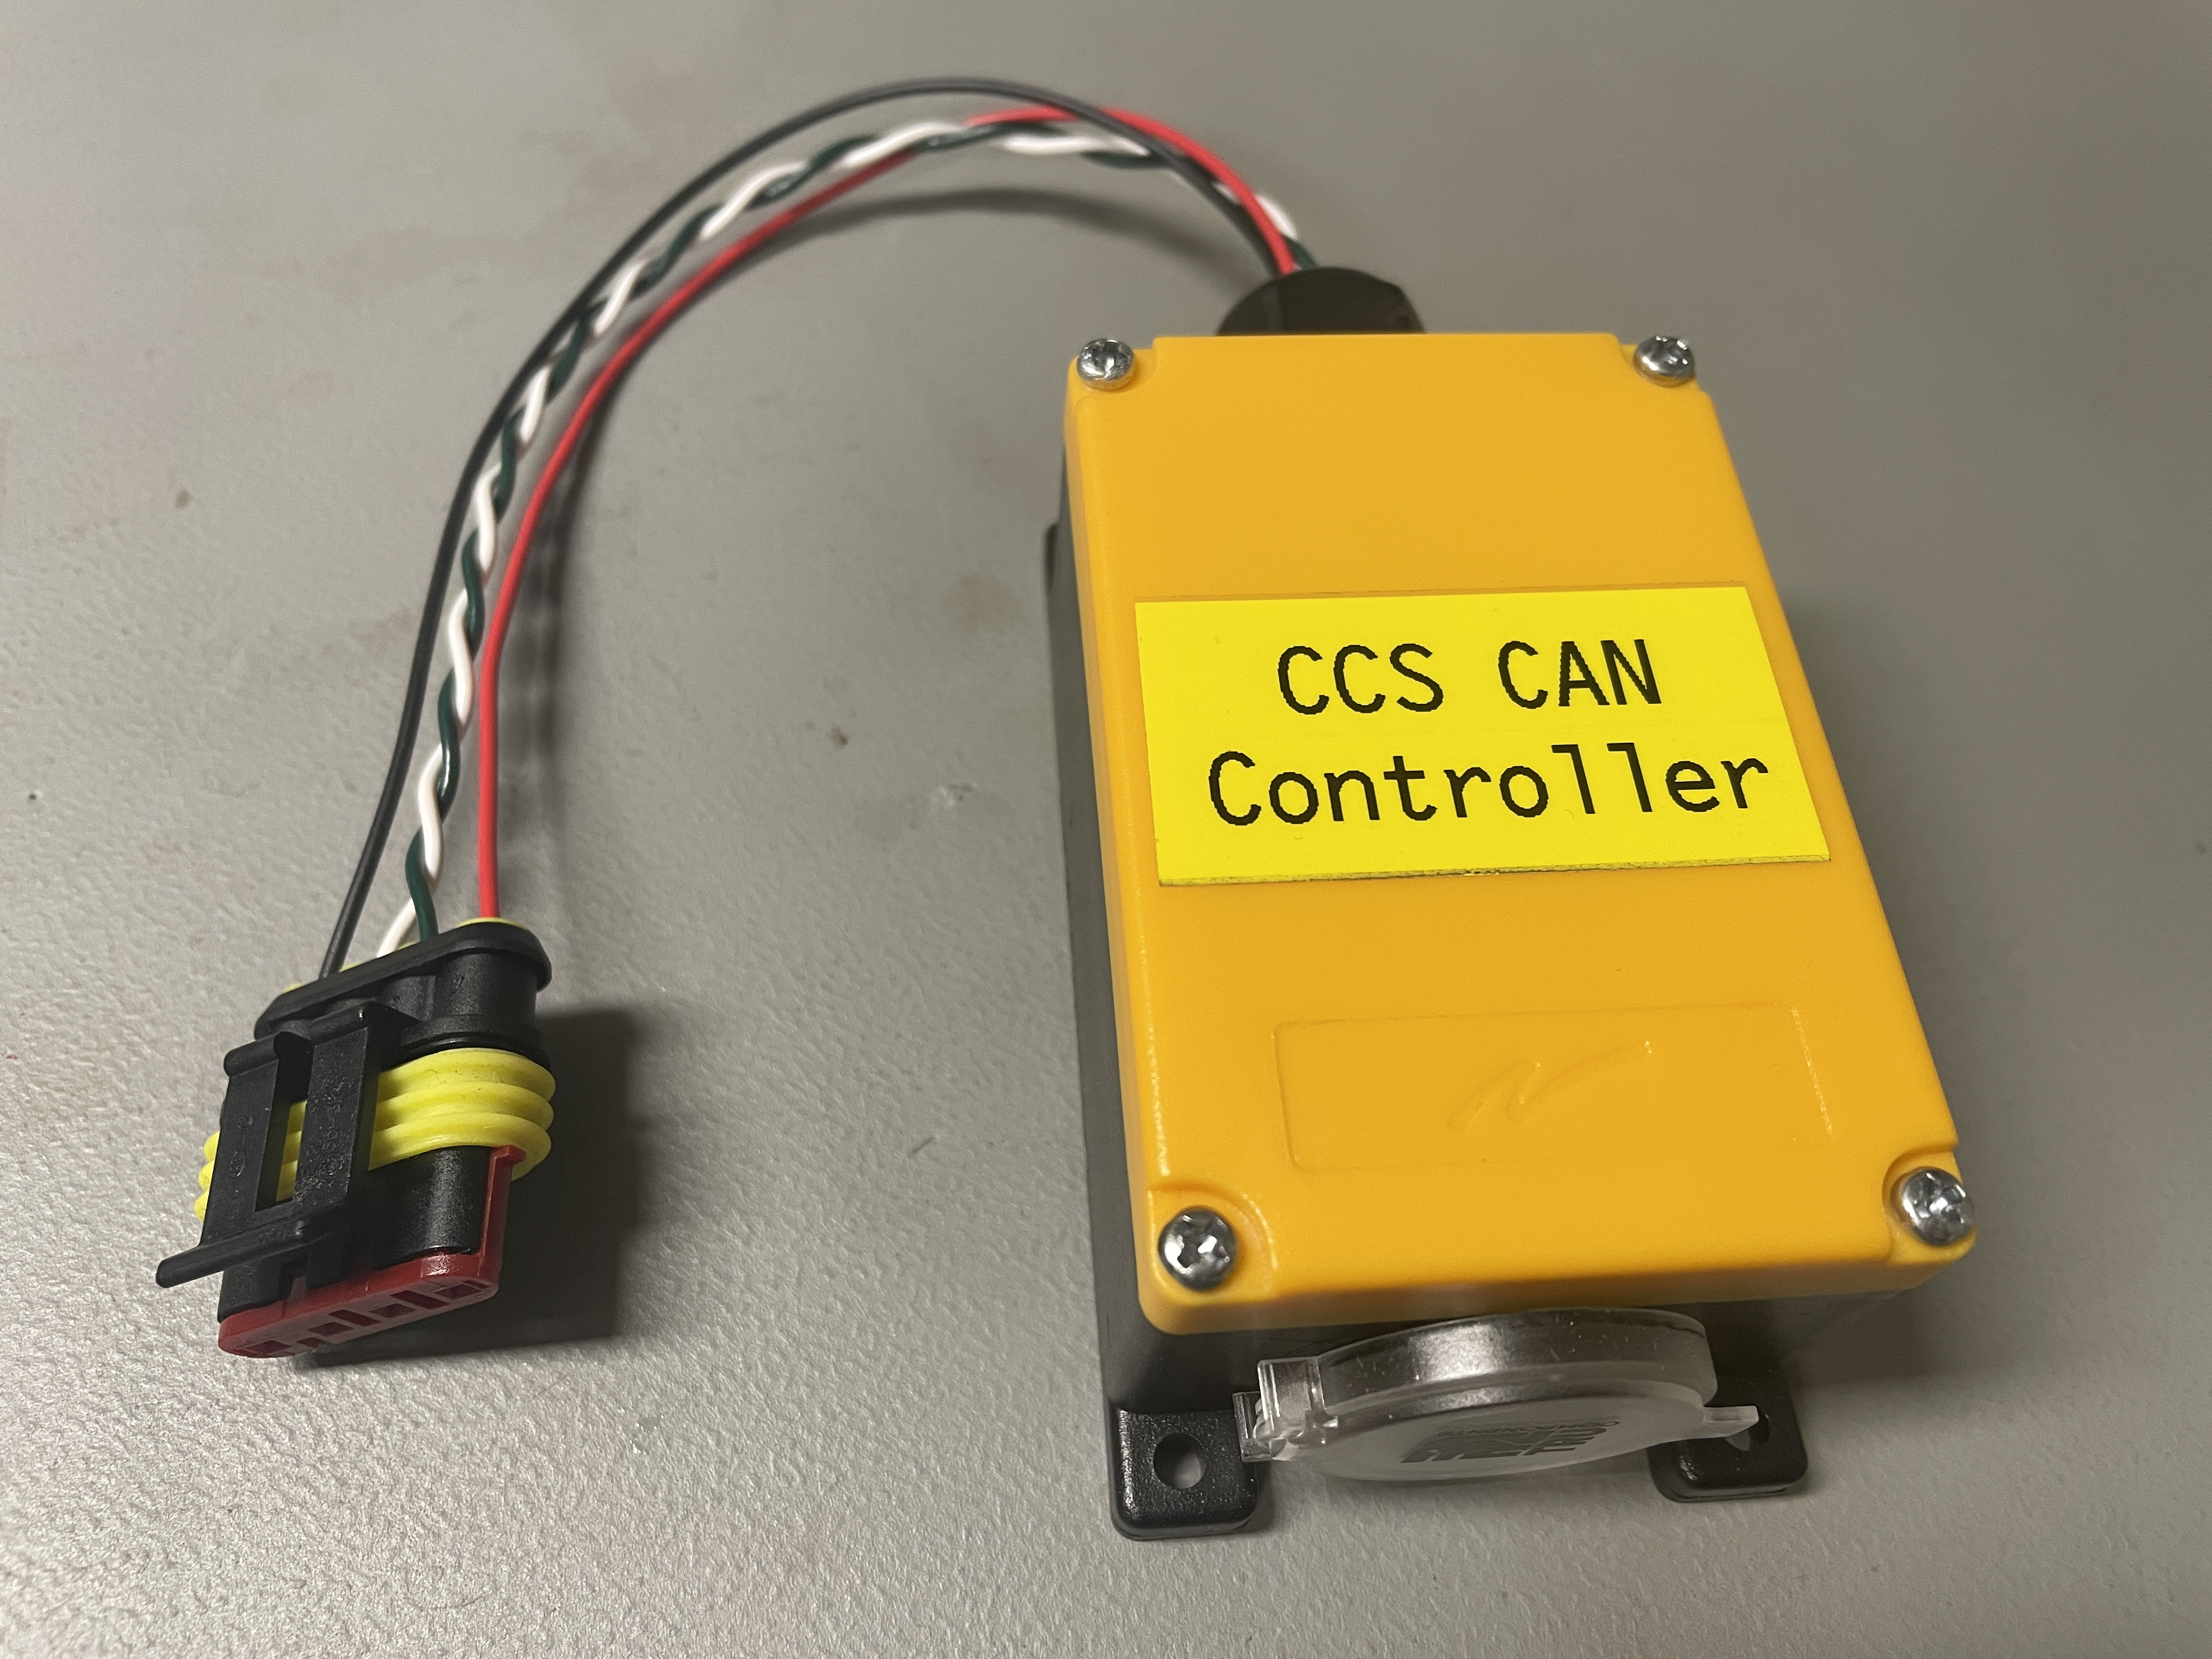
\includegraphics[width=0.9\textwidth]{behuizing}}
        \caption{Behuizing van de CCS CAN controller}
        \label{fig:behuizing}
    \end{minipage}\hfill
    \begin{minipage}{0.45\textwidth}
        \centerline{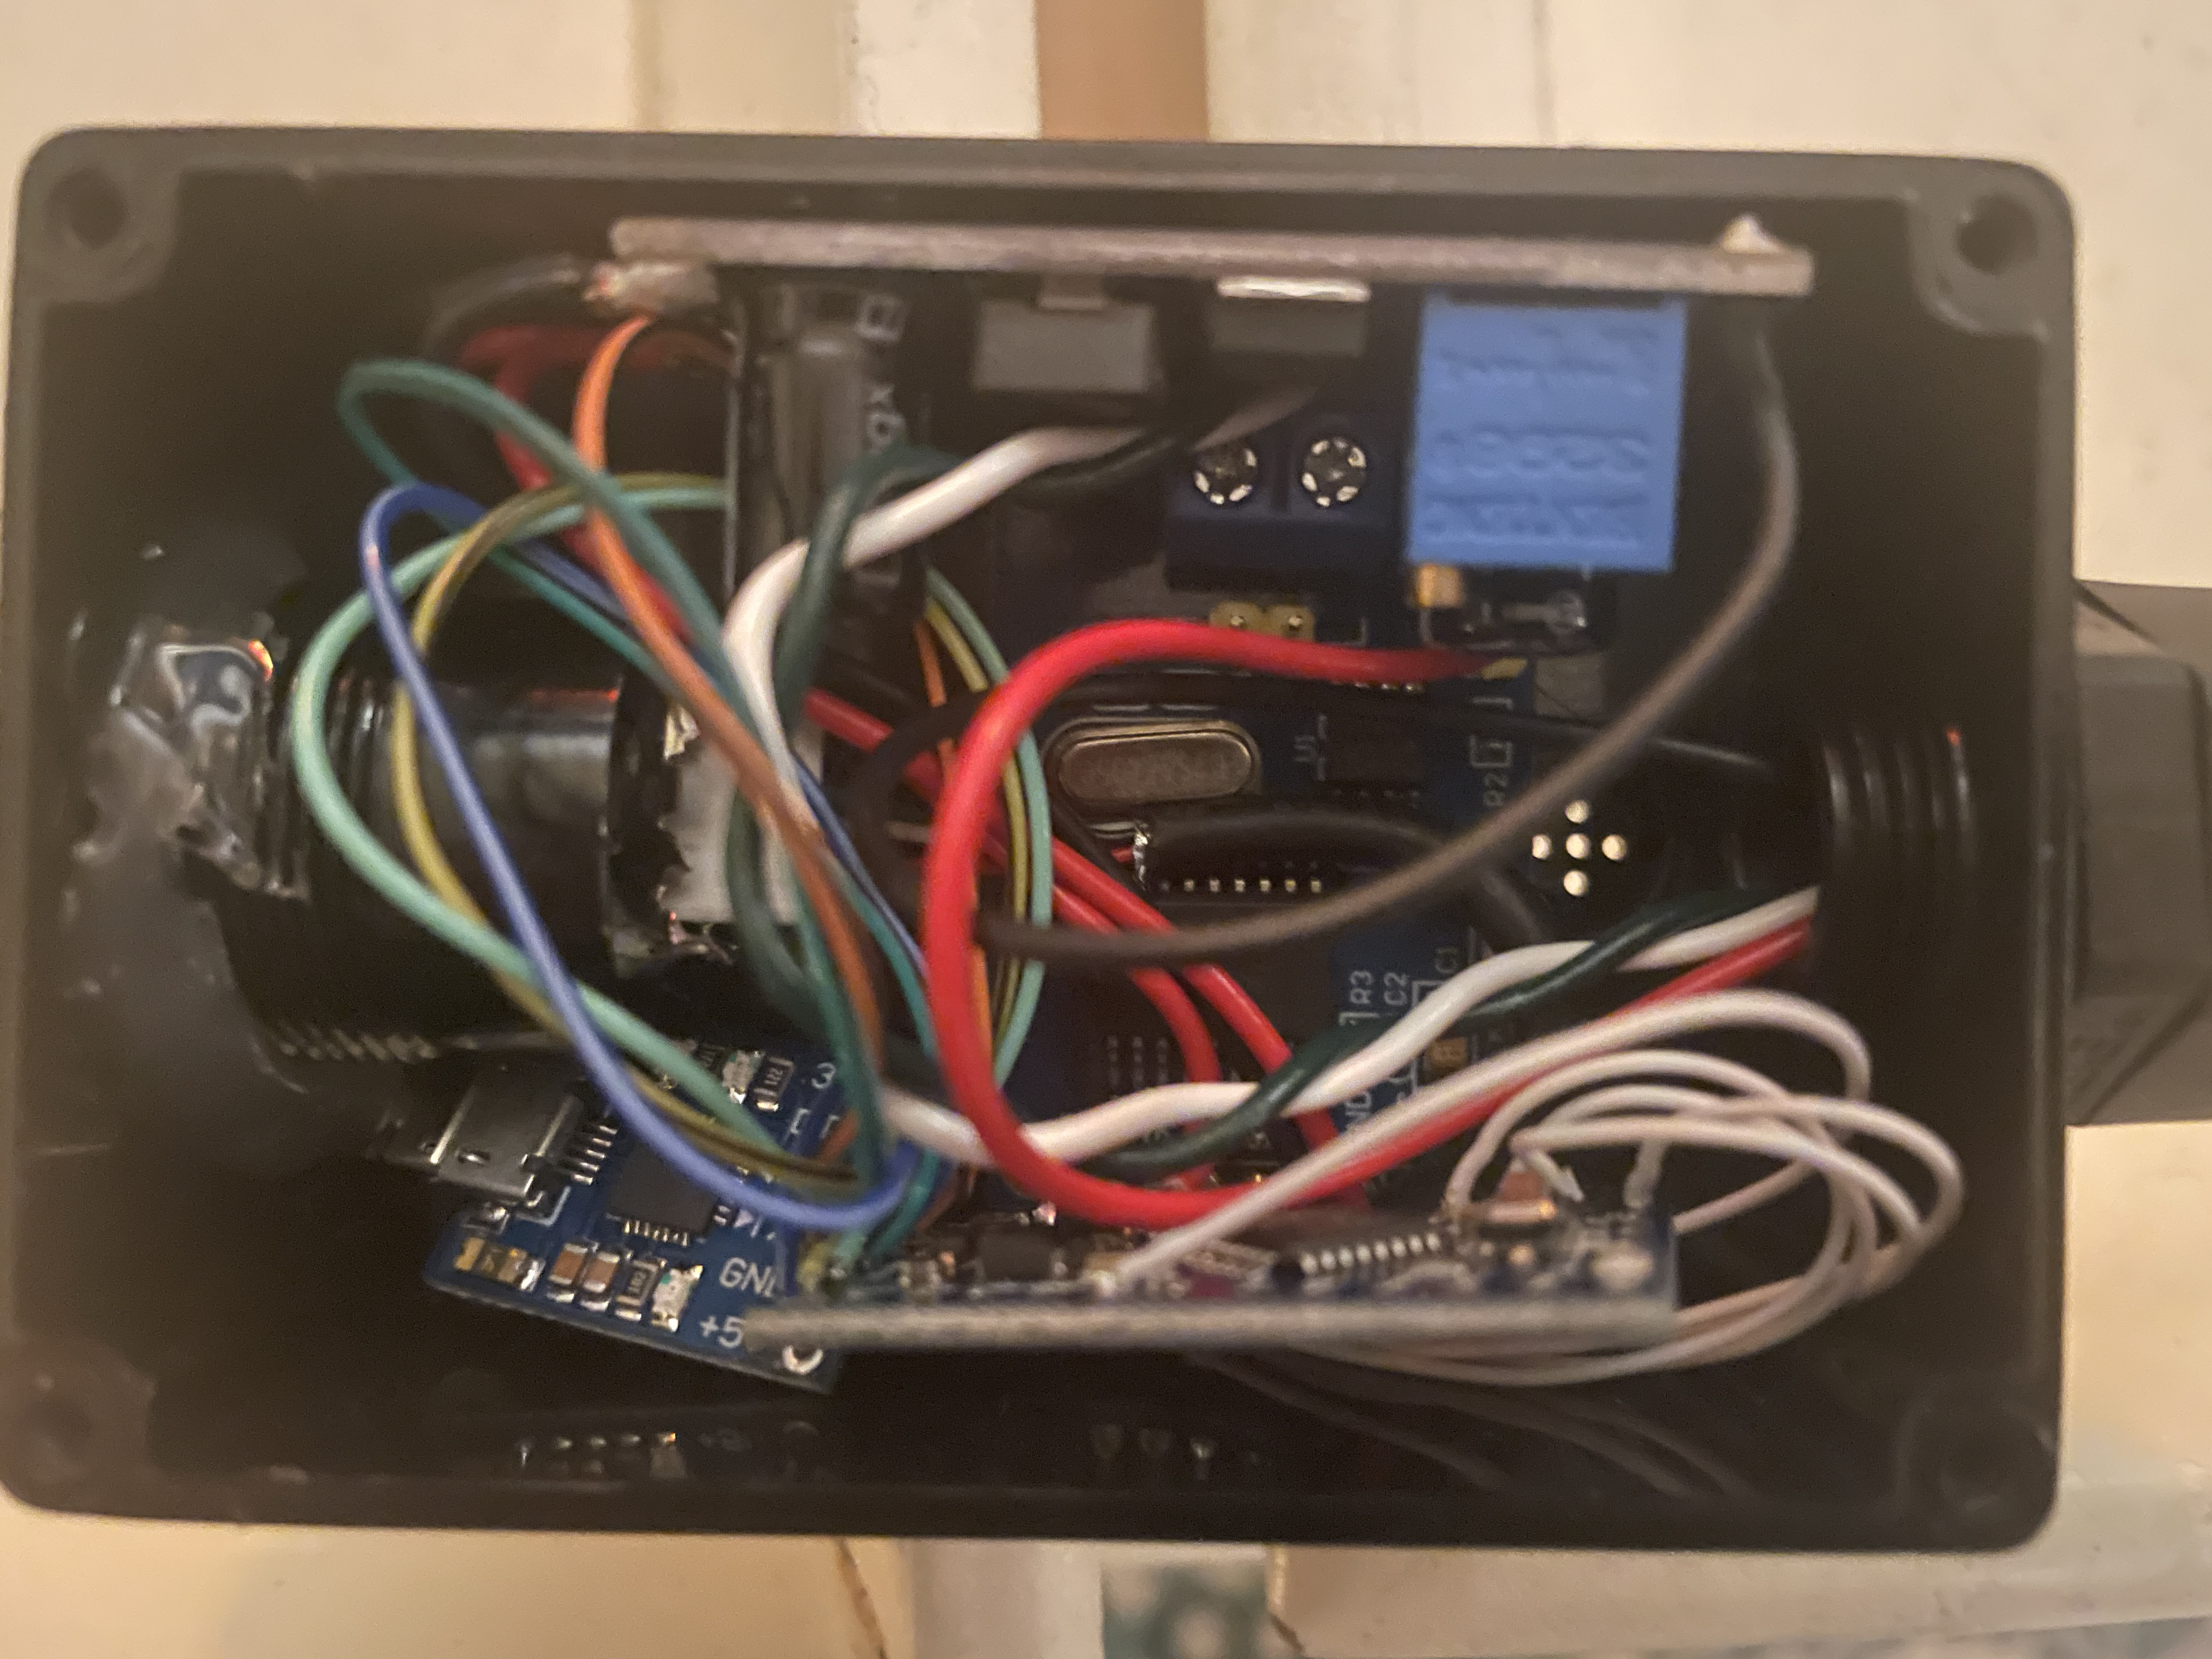
\includegraphics[width=0.9\textwidth]{binnenkant}}
        \caption{Binnenkant van de behuizing}
        \label{fig:binnenkant}
    \end{minipage}
\end{figure}

In figuur \ref{fig:behuizing} is het eindresultaat te zien, een kleine lasdoos
is gebruikt als behuizing, met aan een kant een wartel als doorvoer van de CAN
bus en de \si{12\volt} uit de auto en aan de andere kant een panel mount USB
aansluiting, om de Arduino te kunnen programmeren. In figuur
\ref{fig:binnenkant} is de binnenkant van de behuizing te zien. Het is best
krap aan de binnenkant, maar alles past wel omdat er geen gebruik meer word
gemaakt van headers, maar alle verbindingen zijn direct aan de pcb gesoldeerd.
\chapter{Toetsing eindresultaat aan de hand van de eisen}
\label{Toetsing_eindresultaat_aan_de_hand_van_de_eisen}
%%%%%%%%%%%%%%%%%%%%%%%%%%%%%%%%%%%%%%%%%%%%%%%%%%%%%%%%%%%%%%%%%%%%%%%%

Door een modem van Zero-ev te gebruiken hoeven we ons geen zorgen te maken over
of het aan de betreffende wet- en regelgeving voldoet, dat moet namelijk
allemaal door Zero-ev zijn geregeld. 

Om de overigen eisen te testen, zijn we met de proefopstelling (zie hoofdstuk
\ref{sec:proefopstelling}) langs verschillende CCS-snelladers gegaan. We hebben
getest of: het laden werkt, er ingesteld kan worden wat de gewenste laadstroom
is en of het laden makkelijk gestart en gestopt kan worden. Ook is de
communicatie tussen het BMS en het modem via de CCS CAN-controller getest.



\begin{figure}[]
    \centering
    \begin{minipage}{0.45\textwidth}
        \centerline{\includegraphics[width=0.9\textwidth]{testen1}}
        \caption{Testen van de CCS proefopstelling bij een Fastned snellader}
        \label{fig:testen1}
    \end{minipage}\hfill
    \begin{minipage}{0.45\textwidth}
        \centerline{\includegraphics[width=0.9\textwidth]{testen2}}
        \caption{Testen van de CCS proefopstelling bij een Allego snellader}
        \label{fig:testen2}
    \end{minipage}
\end{figure}
\chapter{Conclusie en aanbevelingen}
\label{Conclusie_en_aanbevelingen}
%%%%%%%%%%%%%%%%%%%%%%%%%%%%%%%%%%%%%%%%%%%%%%%%%%%%%%%%%%%%%%%%%%%%%%%%

Uit dit verslag kan geconcludeerd woorden dat dit project geslaagd is omdat het
product op tijd werd opgeleverd, en voldoet aan alle gestelden eisen.

Echter zijn er wel wat aandachtpunten, zoals dat de printqwalitijd niet voledig
naar wens is, daarvoor is de aanbeveling aan 3devo om:

\begin{itemize}
    \item Een gewater koelde extruder te installeren
    \item De printer beter te tunen om met gewenste kwaliteit te printen.
\end{itemize}
% \chapter{Evaluatie}
\label{Evaluatie}
%%%%%%%%%%%%%%%%%%%%%%%%%%%%%%%%%%%%%%%%%%%%%%%%%%%%%%%%%%%%%%%%%%%%%%%%

%%%%%%%%%%%%%%%%%%%%%%%%%%%%%%%%%%%%%%%%%%%%%%%%%%%%%%%%%%%%%%%%%%%%%%%%
% \section{Section}
%%%%%%%%%%%%%%%%%%%%%%%%%%%%%%%%%%%%%%%%%%%%%%%%%%%%%%%%%%%%%%%%%%%%%%%%

%%%%%%%%%%%%%%%%%%%%%%%%%%%%%%%%%%%%%%%%%%%%%%%%%%%%%%%%%%%%%%%%%%%%%%%%
% \subsection{Subsection}
%%%%%%%%%%%%%%%%%%%%%%%%%%%%%%%%%%%%%%%%%%%%%%%%%%%%%%%%%%%%%%%%%%%%%%%%



% This ensures that the subsequent sections are being included as root
% items in the bookmark structure of your PDF reader.
\bookmarksetup{startatroot}

\bibliographystyle{IEEEtran}
\bibliography{bronnen}

\begin{appendices}
\appendixpage
\noappendicestocpagenum
\addappheadtotoc
\chapter{Intervisie}
\includepdf[pages=-,fitpaper,rotateoversize]{Appendices/Intervisie/Intervisie.pdf}
\chapter{Student over docentbezoek}
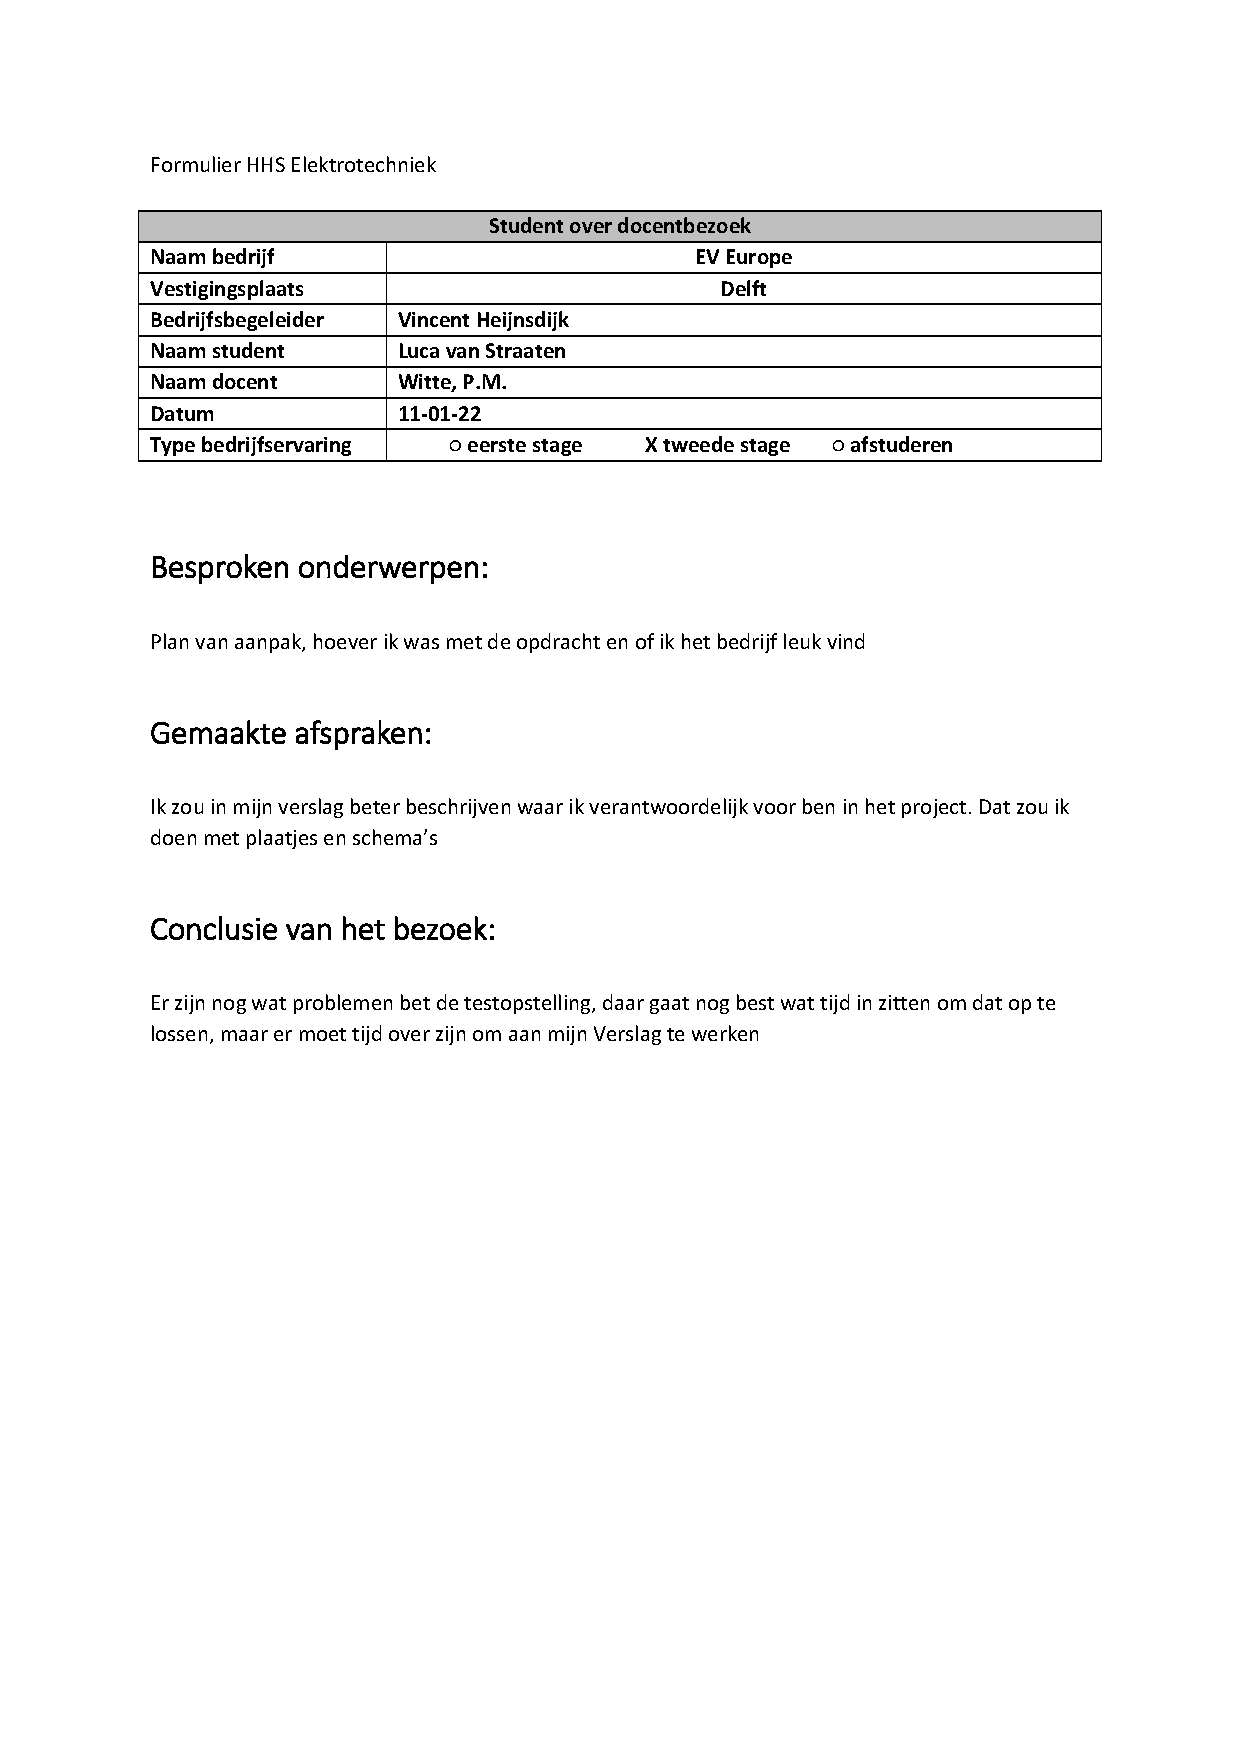
\includepdf[pages=-,fitpaper,rotateoversize]{Appendices/student_over_docentbezoek.pdf}
\chapter{Bedrijf over student}
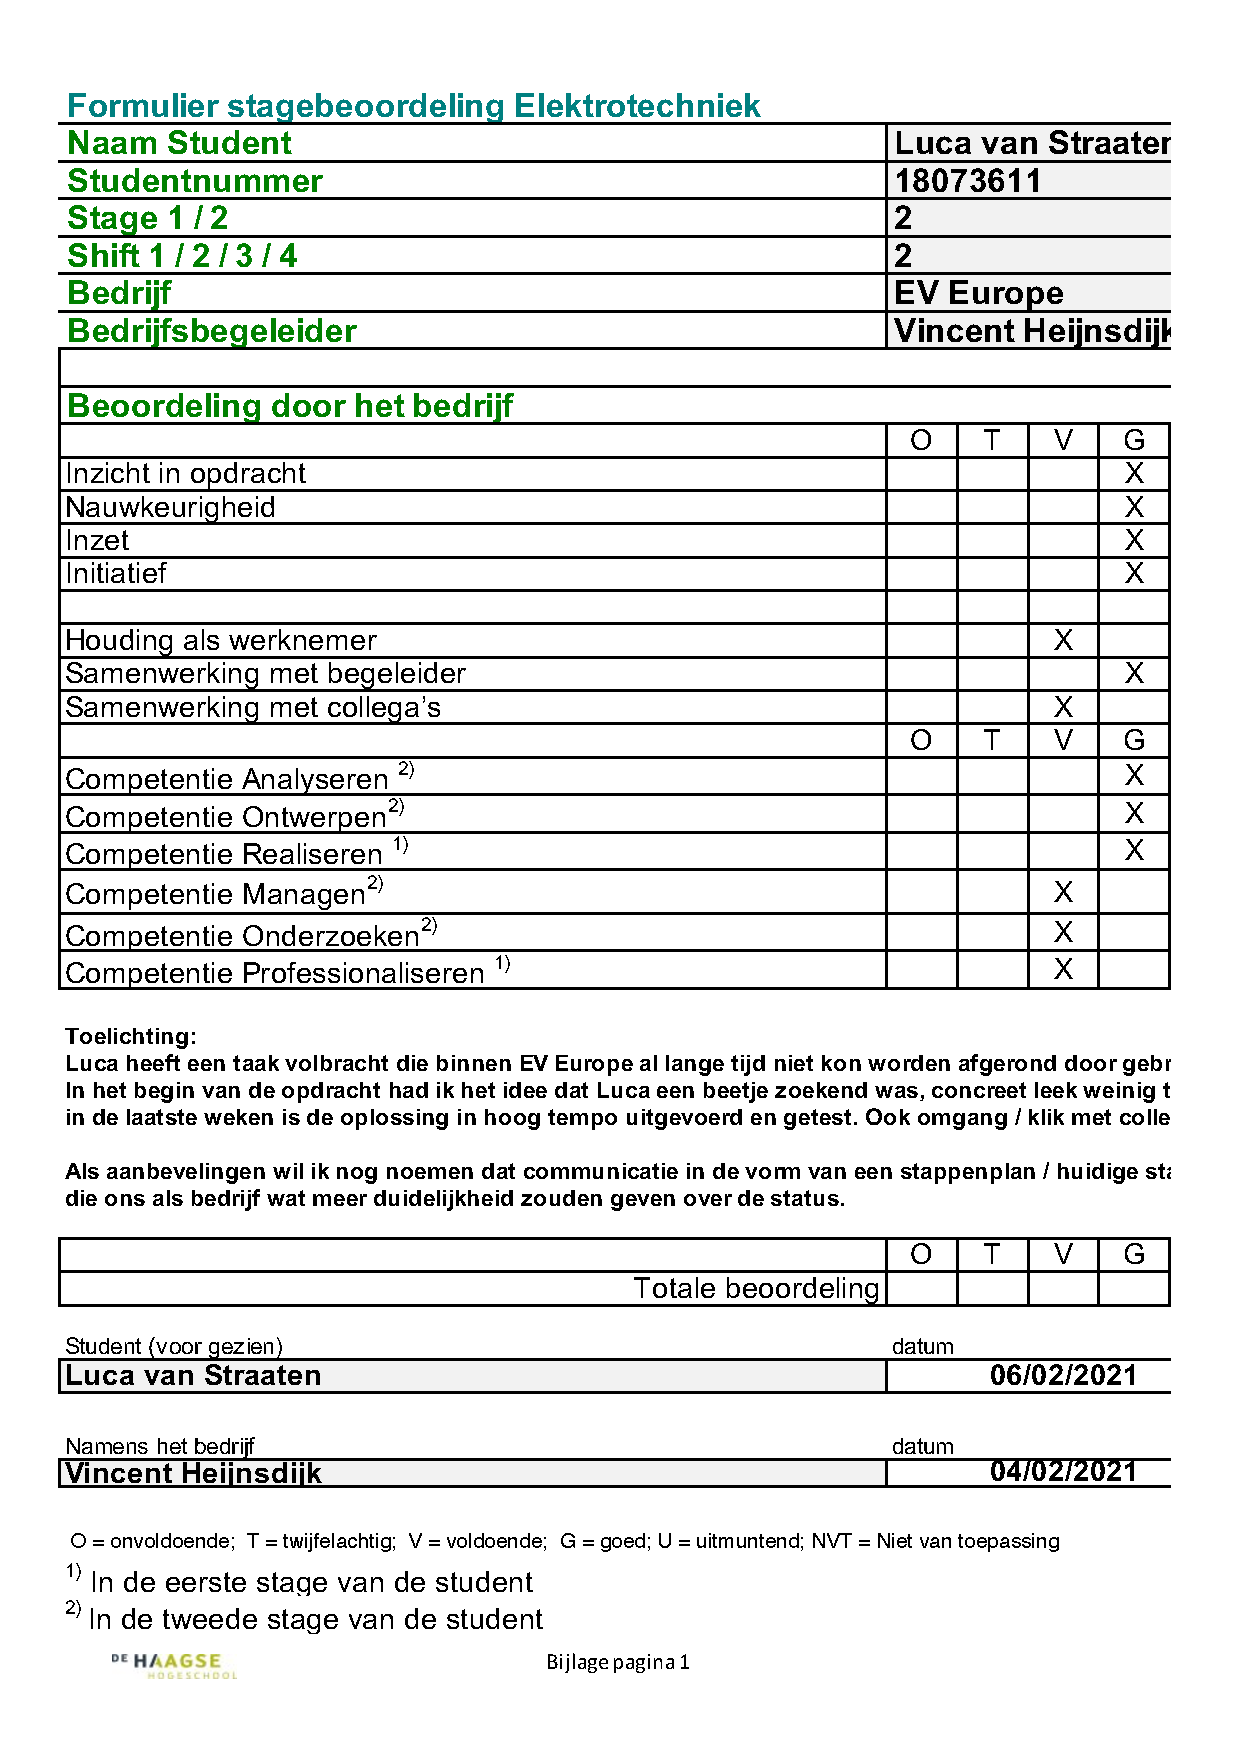
\includepdf[pages=-,fitpaper,rotateoversize]{Appendices/Bedrijf_over_student.pdf}
\chapter{Student over bedrijf}
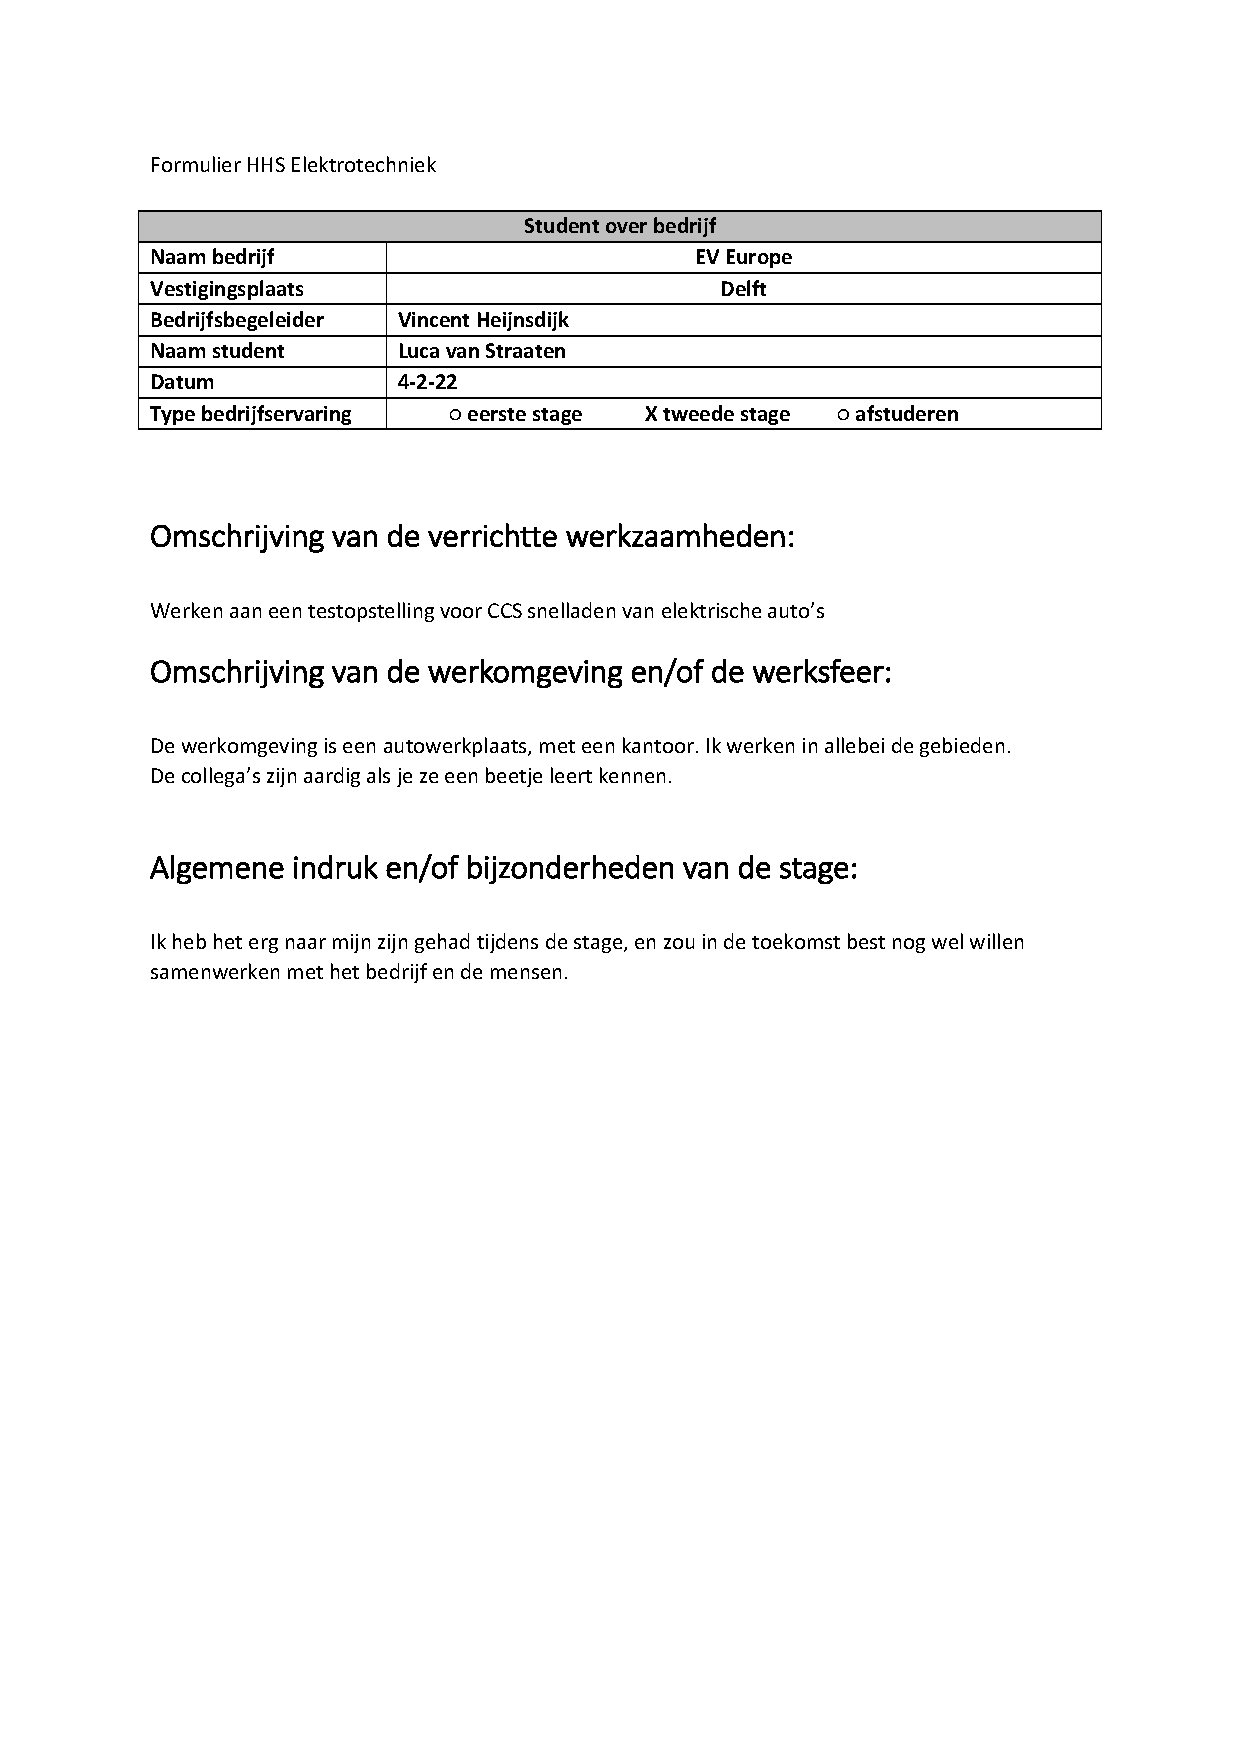
\includepdf[pages=-,fitpaper,rotateoversize]{Appendices/student_over_bedrijf/student_over_bedrijf.pdf}
\chapter{Verantwoording van de behaalde competenties}
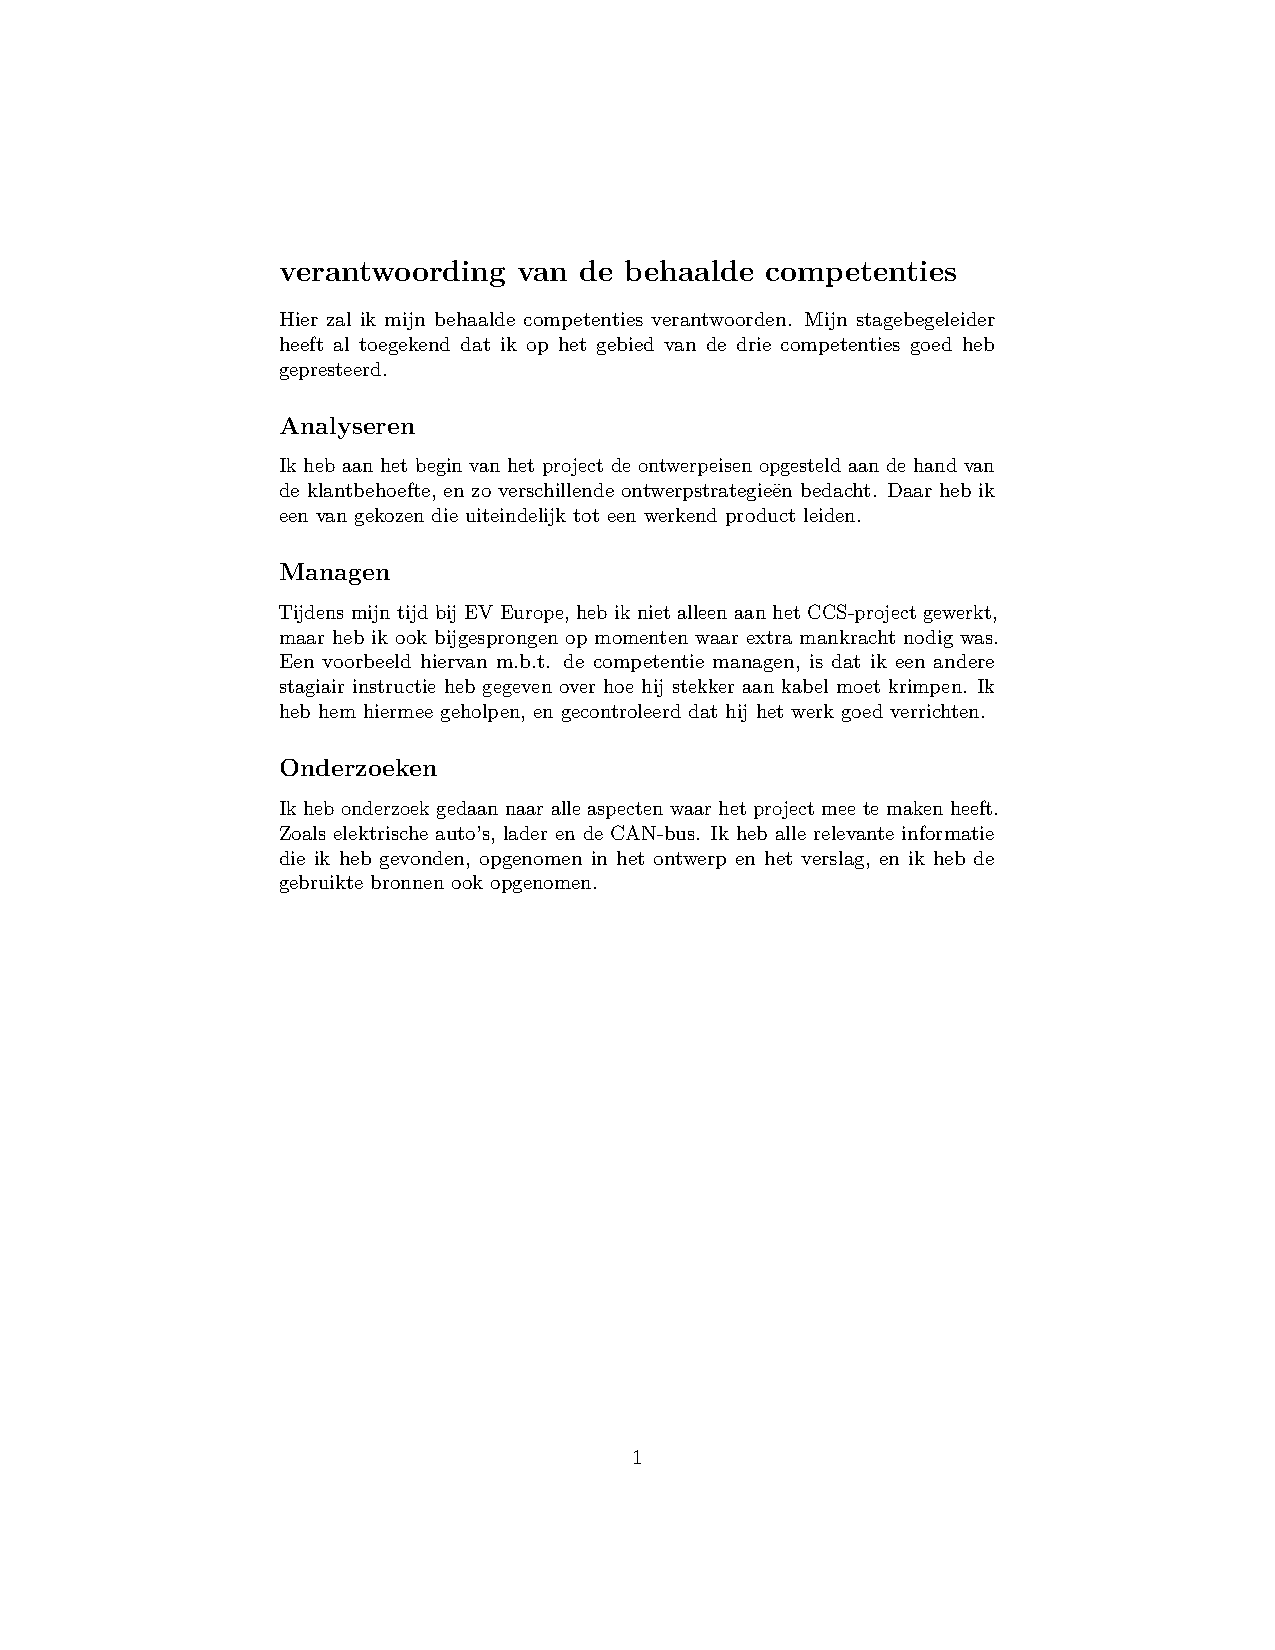
\includepdf[pages=-,fitpaper,rotateoversize]{Appendices/Verantwoording_behaalde_competenties/competenties.pdf}
\chapter{korte beschrijving van de bedrijfsorganisatie}
\includepdf[pages=-,fitpaper,rotateoversize]{Appendices/Bedrijfsorganisatie/organisatie.pdf}
\chapter{overdracht document}
\label{overdracht}
\includepdf[pages=-,fitpaper,rotateoversize]{Appendices/overdracht.pdf}
\end{appendices}

\backmatter
\end{document}
